\documentclass{article}%
\usepackage[T1]{fontenc}%
\usepackage[utf8]{inputenc}%
\usepackage{lmodern}%
\usepackage{textcomp}%
\usepackage{lastpage}%
\usepackage{float}%
\usepackage{graphicx}%
\usepackage{booktabs}%
\usepackage{geometry}%
\geometry{margin=2.5cm}%
%
\title{Auswertung der Fahrraddaten}%
\author{}%
\date{\today}%
%
\begin{document}%
\normalsize%
\maketitle%
\section{Berechnete Kennwerte}%
\label{sec:BerechneteKennwerte}%
\begin{tabular}{lr}%
\hline%
\textbf{Kennwert}&\textbf{Wert}\\%
\hline%
Gesamtstrecke&94267.5 m\\%
Durchschnittsgeschwindigkeit&9.24 m/s\\%
Maximalleistung&726.4 W\\%
Gesamtzeit&0 days 04:32:52.391000\\%
Gesamter Anstieg&1095.9 m\\%
Gesamter Abstieg&1097.1 m\\%
Besuchte Orte in Reihenfolge:&{[}'Kufstein', 'Vorderthiersee', 'Mitterland', 'Hinterthiersee', 'Landl', 'Schmiedtal', 'Vorderthiersee', 'Thiersee', 'Kufstein', 'Unterlangkampfen', 'Niederbreitenbach', 'Embach', 'Schönau', 'Breitenbach am Inn', 'Kramsach', 'Kundl', 'Breitenbach am Inn', 'Schönau', 'Achleit', 'Angath', 'Oberlangkampfen', 'Kirchbichl', 'Kufstein'{]}\\%
\hline%
\end{tabular}

%
\section{Diagramme}%
\label{sec:Diagramme}%
\subsection{I\_motor}%
\label{subsec:Imotor}%


\begin{figure}[H]%
\centering%
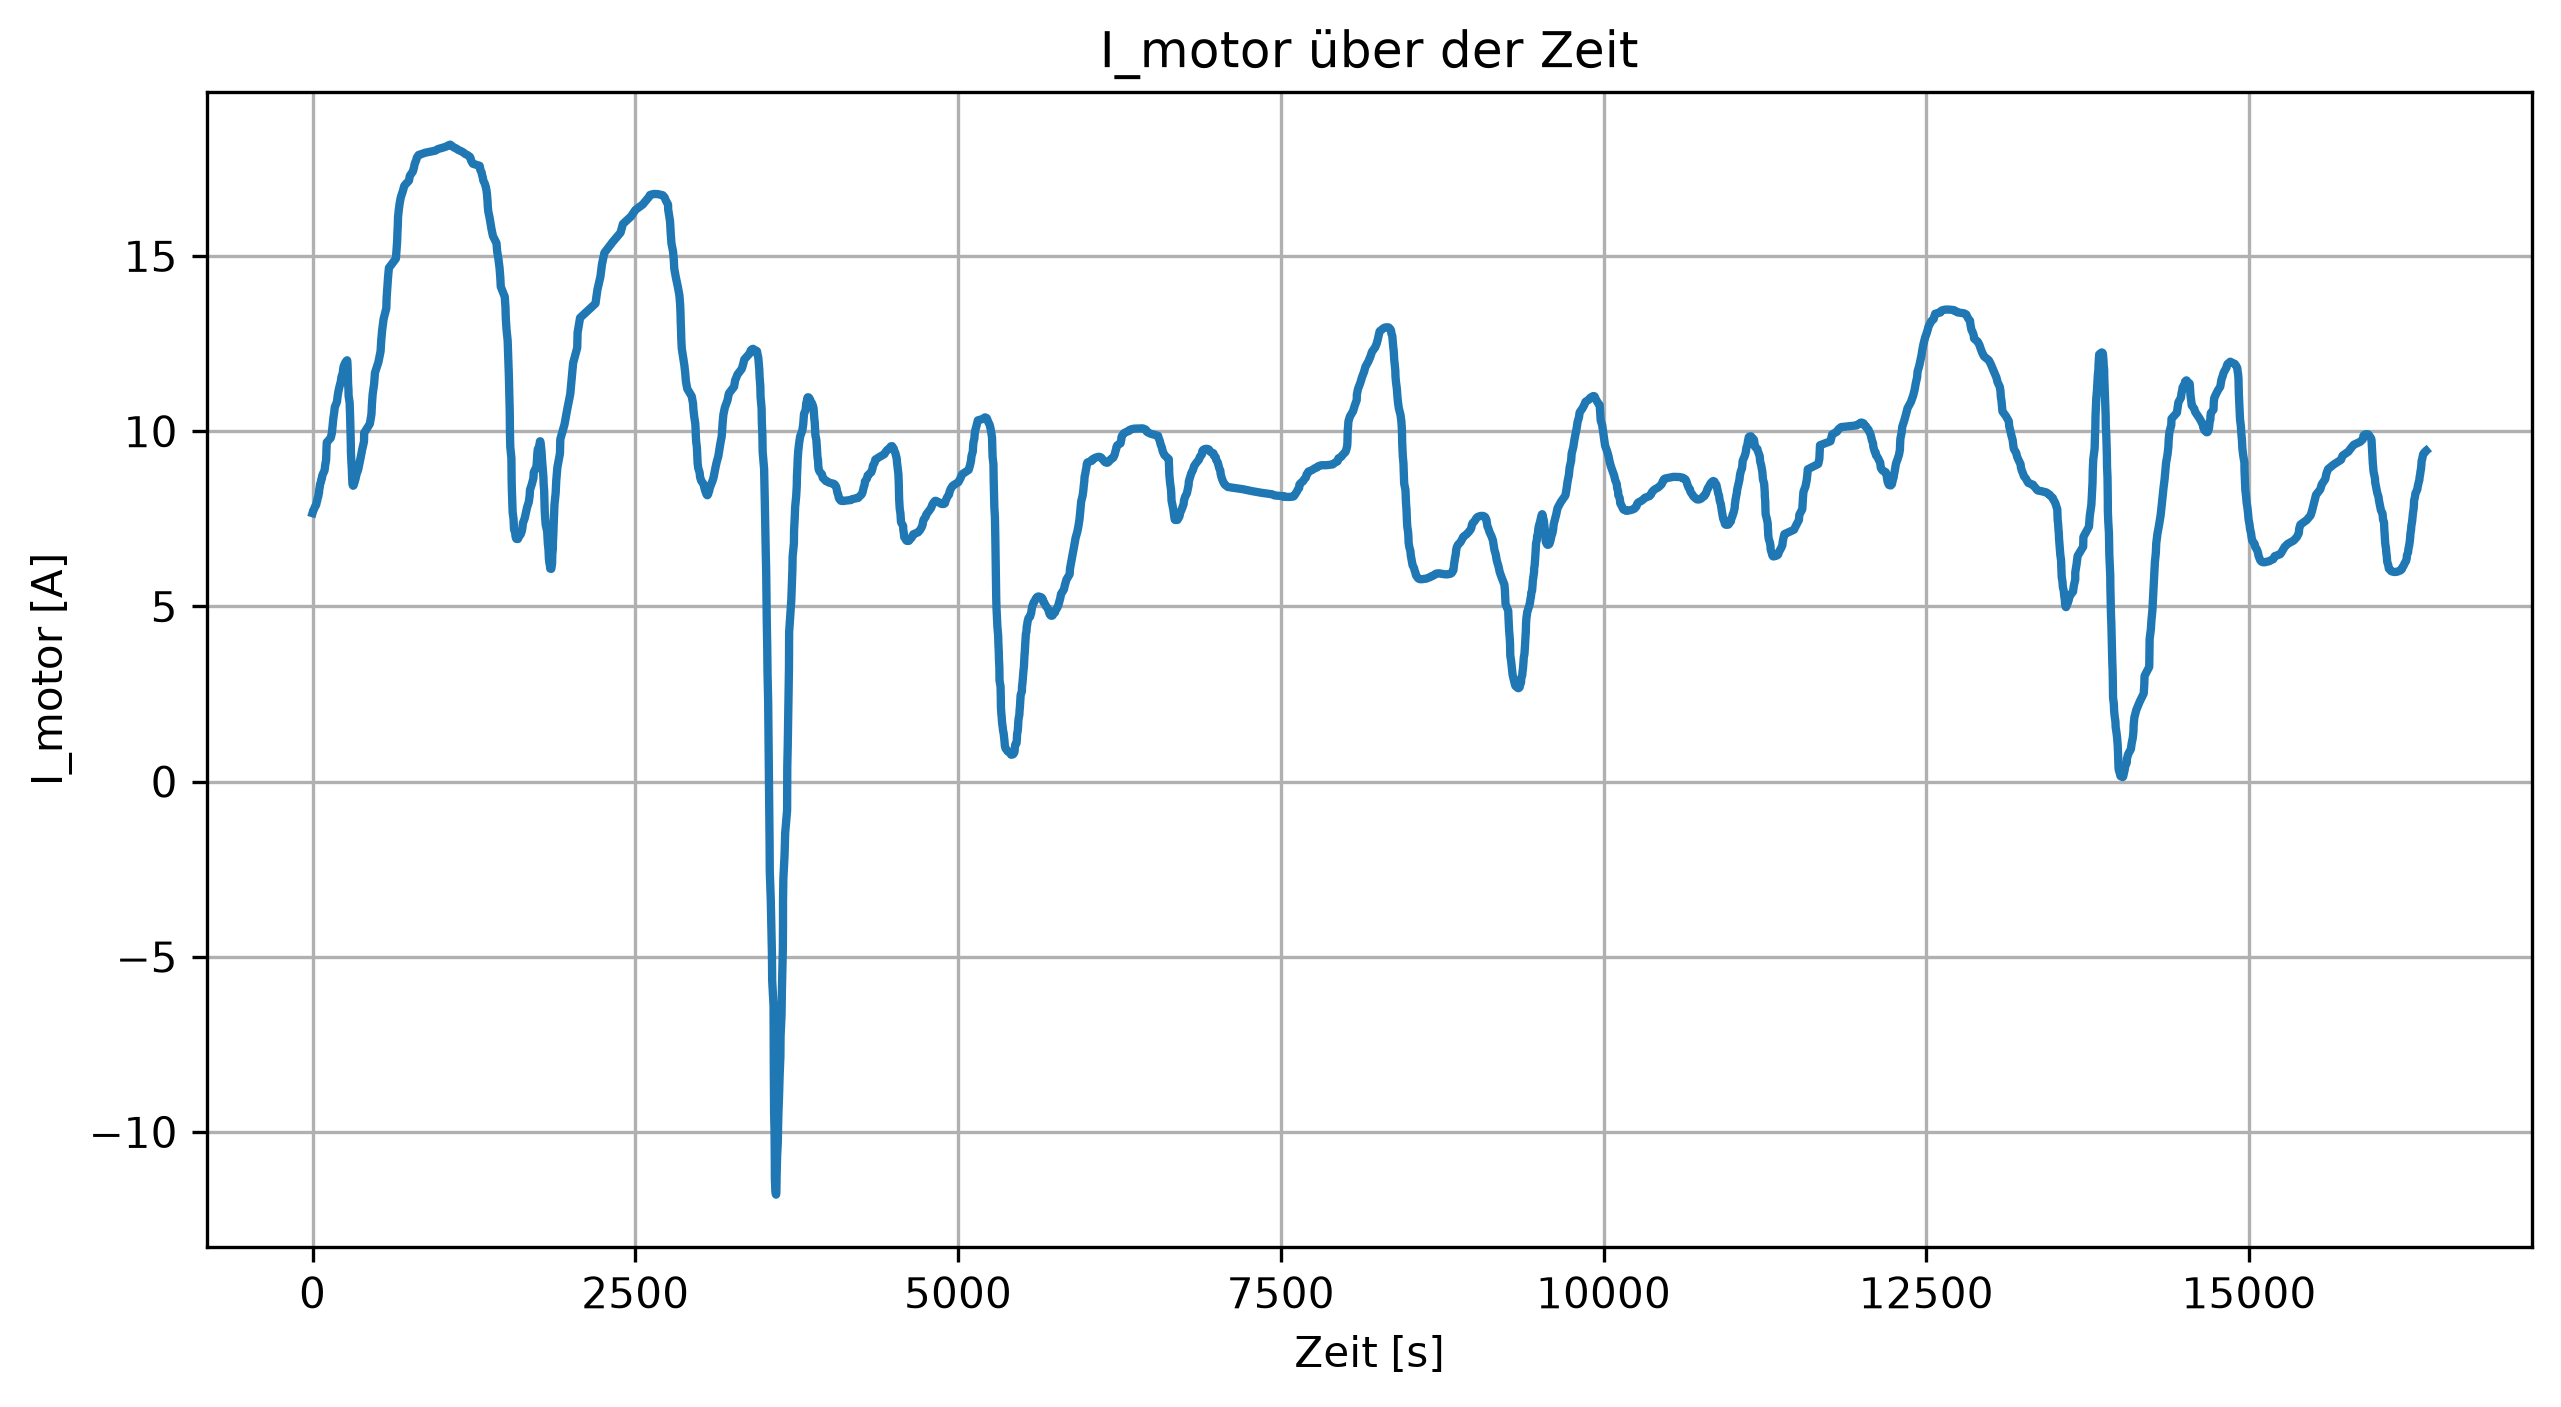
\includegraphics[width=0.95\textwidth]{I_motor.png}%
\caption{I\_motor}%
\end{figure}

%
\subsection{P}%
\label{subsec:P}%


\begin{figure}[H]%
\centering%
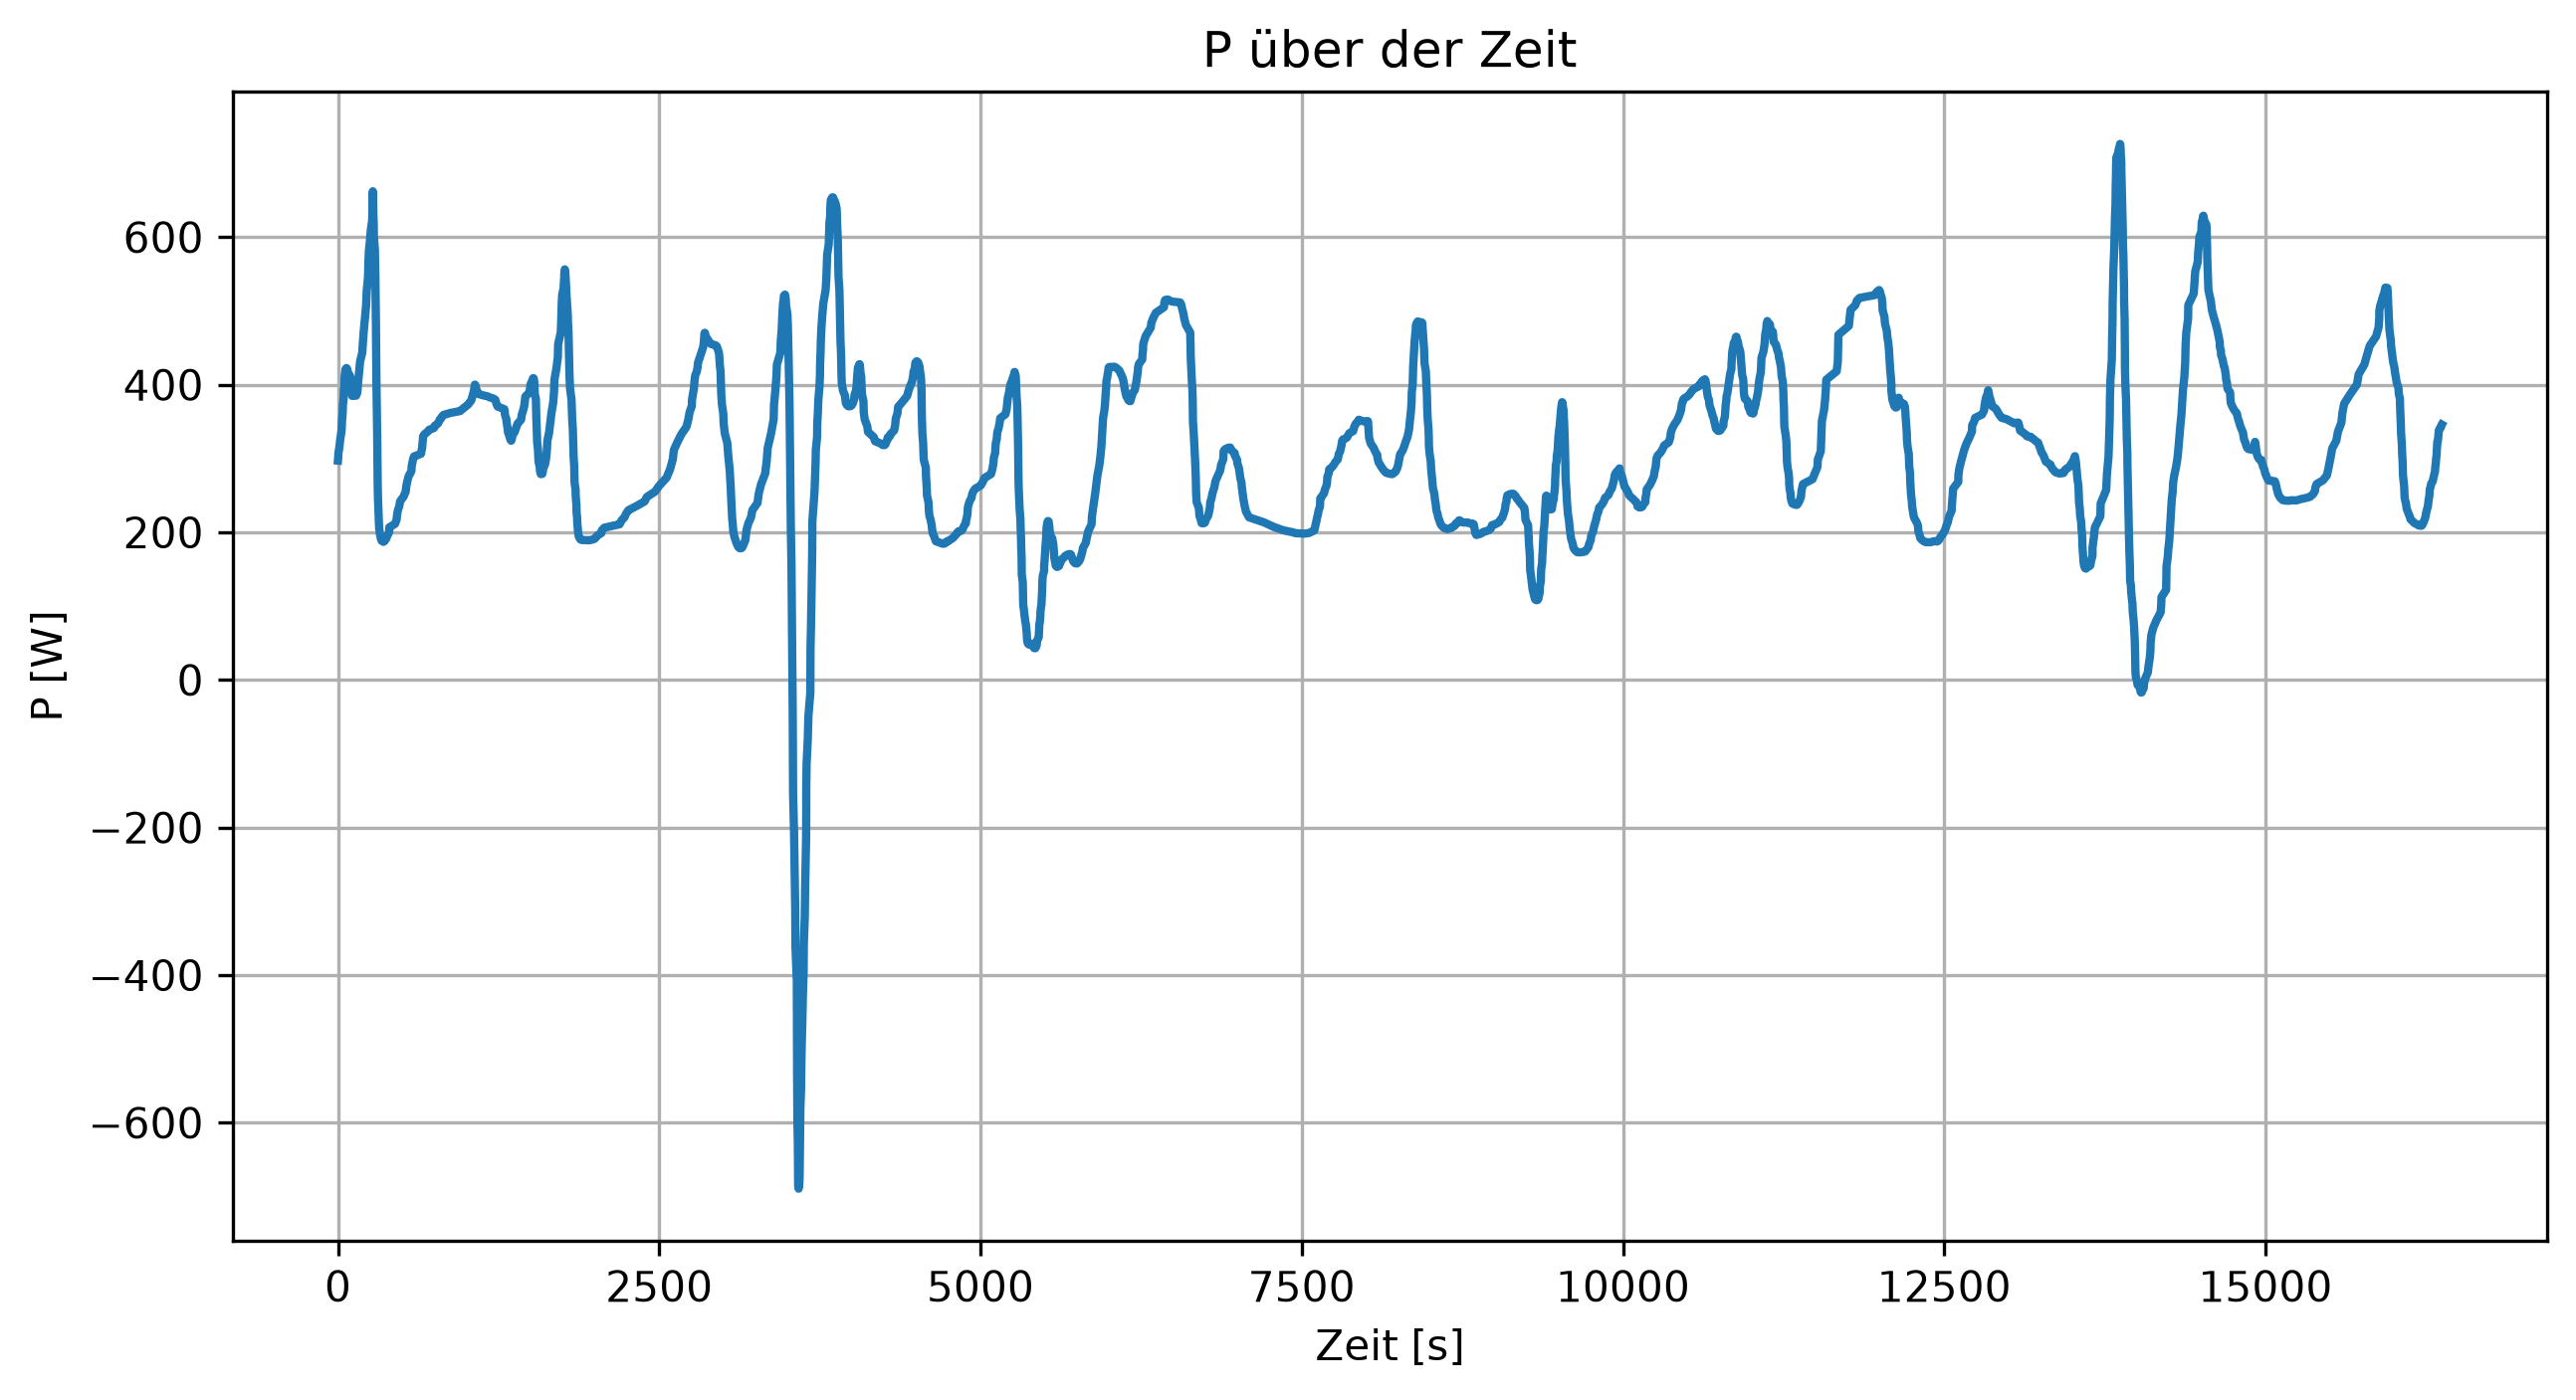
\includegraphics[width=0.95\textwidth]{P.png}%
\caption{P}%
\end{figure}

%
\subsection{Parameterstudie\_A\_P\_max}%
\label{subsec:ParameterstudieAPmax}%


\begin{figure}[H]%
\centering%
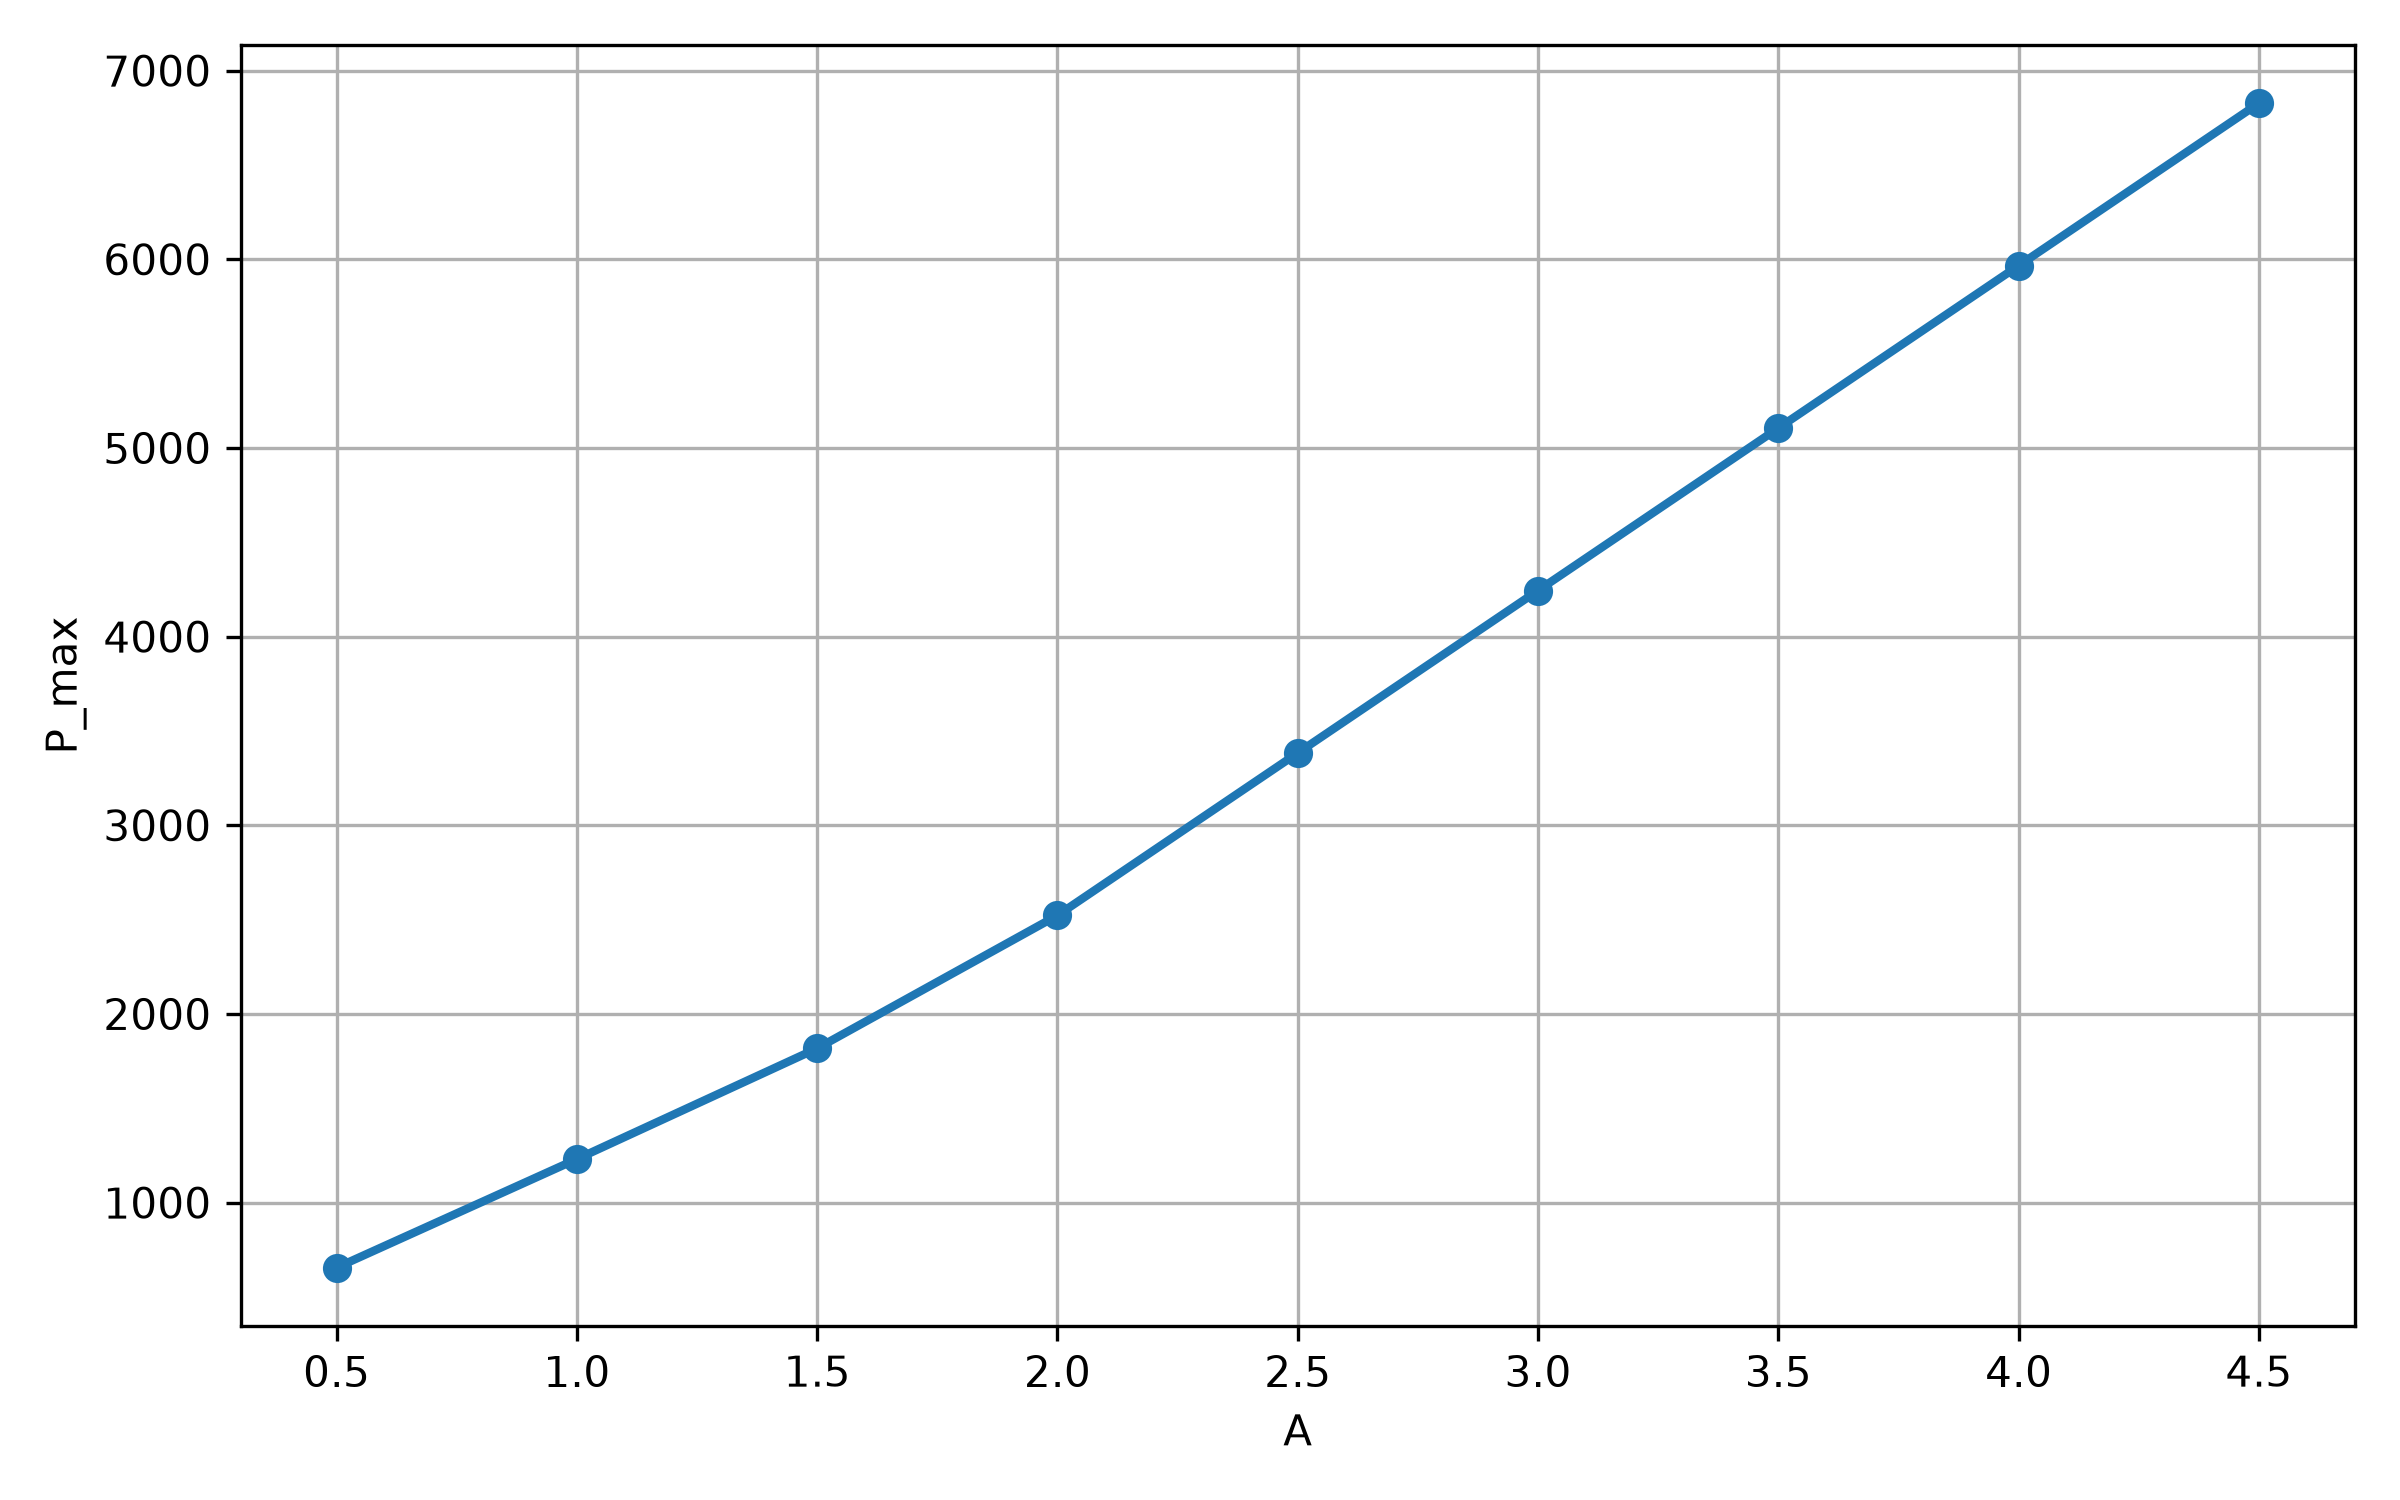
\includegraphics[width=0.95\textwidth]{Parameterstudie_A_P_max.png}%
\caption{Parameterstudie\_A\_P\_max}%
\end{figure}

%
\subsection{Parameterstudie\_masse\_P\_max}%
\label{subsec:ParameterstudiemassePmax}%


\begin{figure}[H]%
\centering%
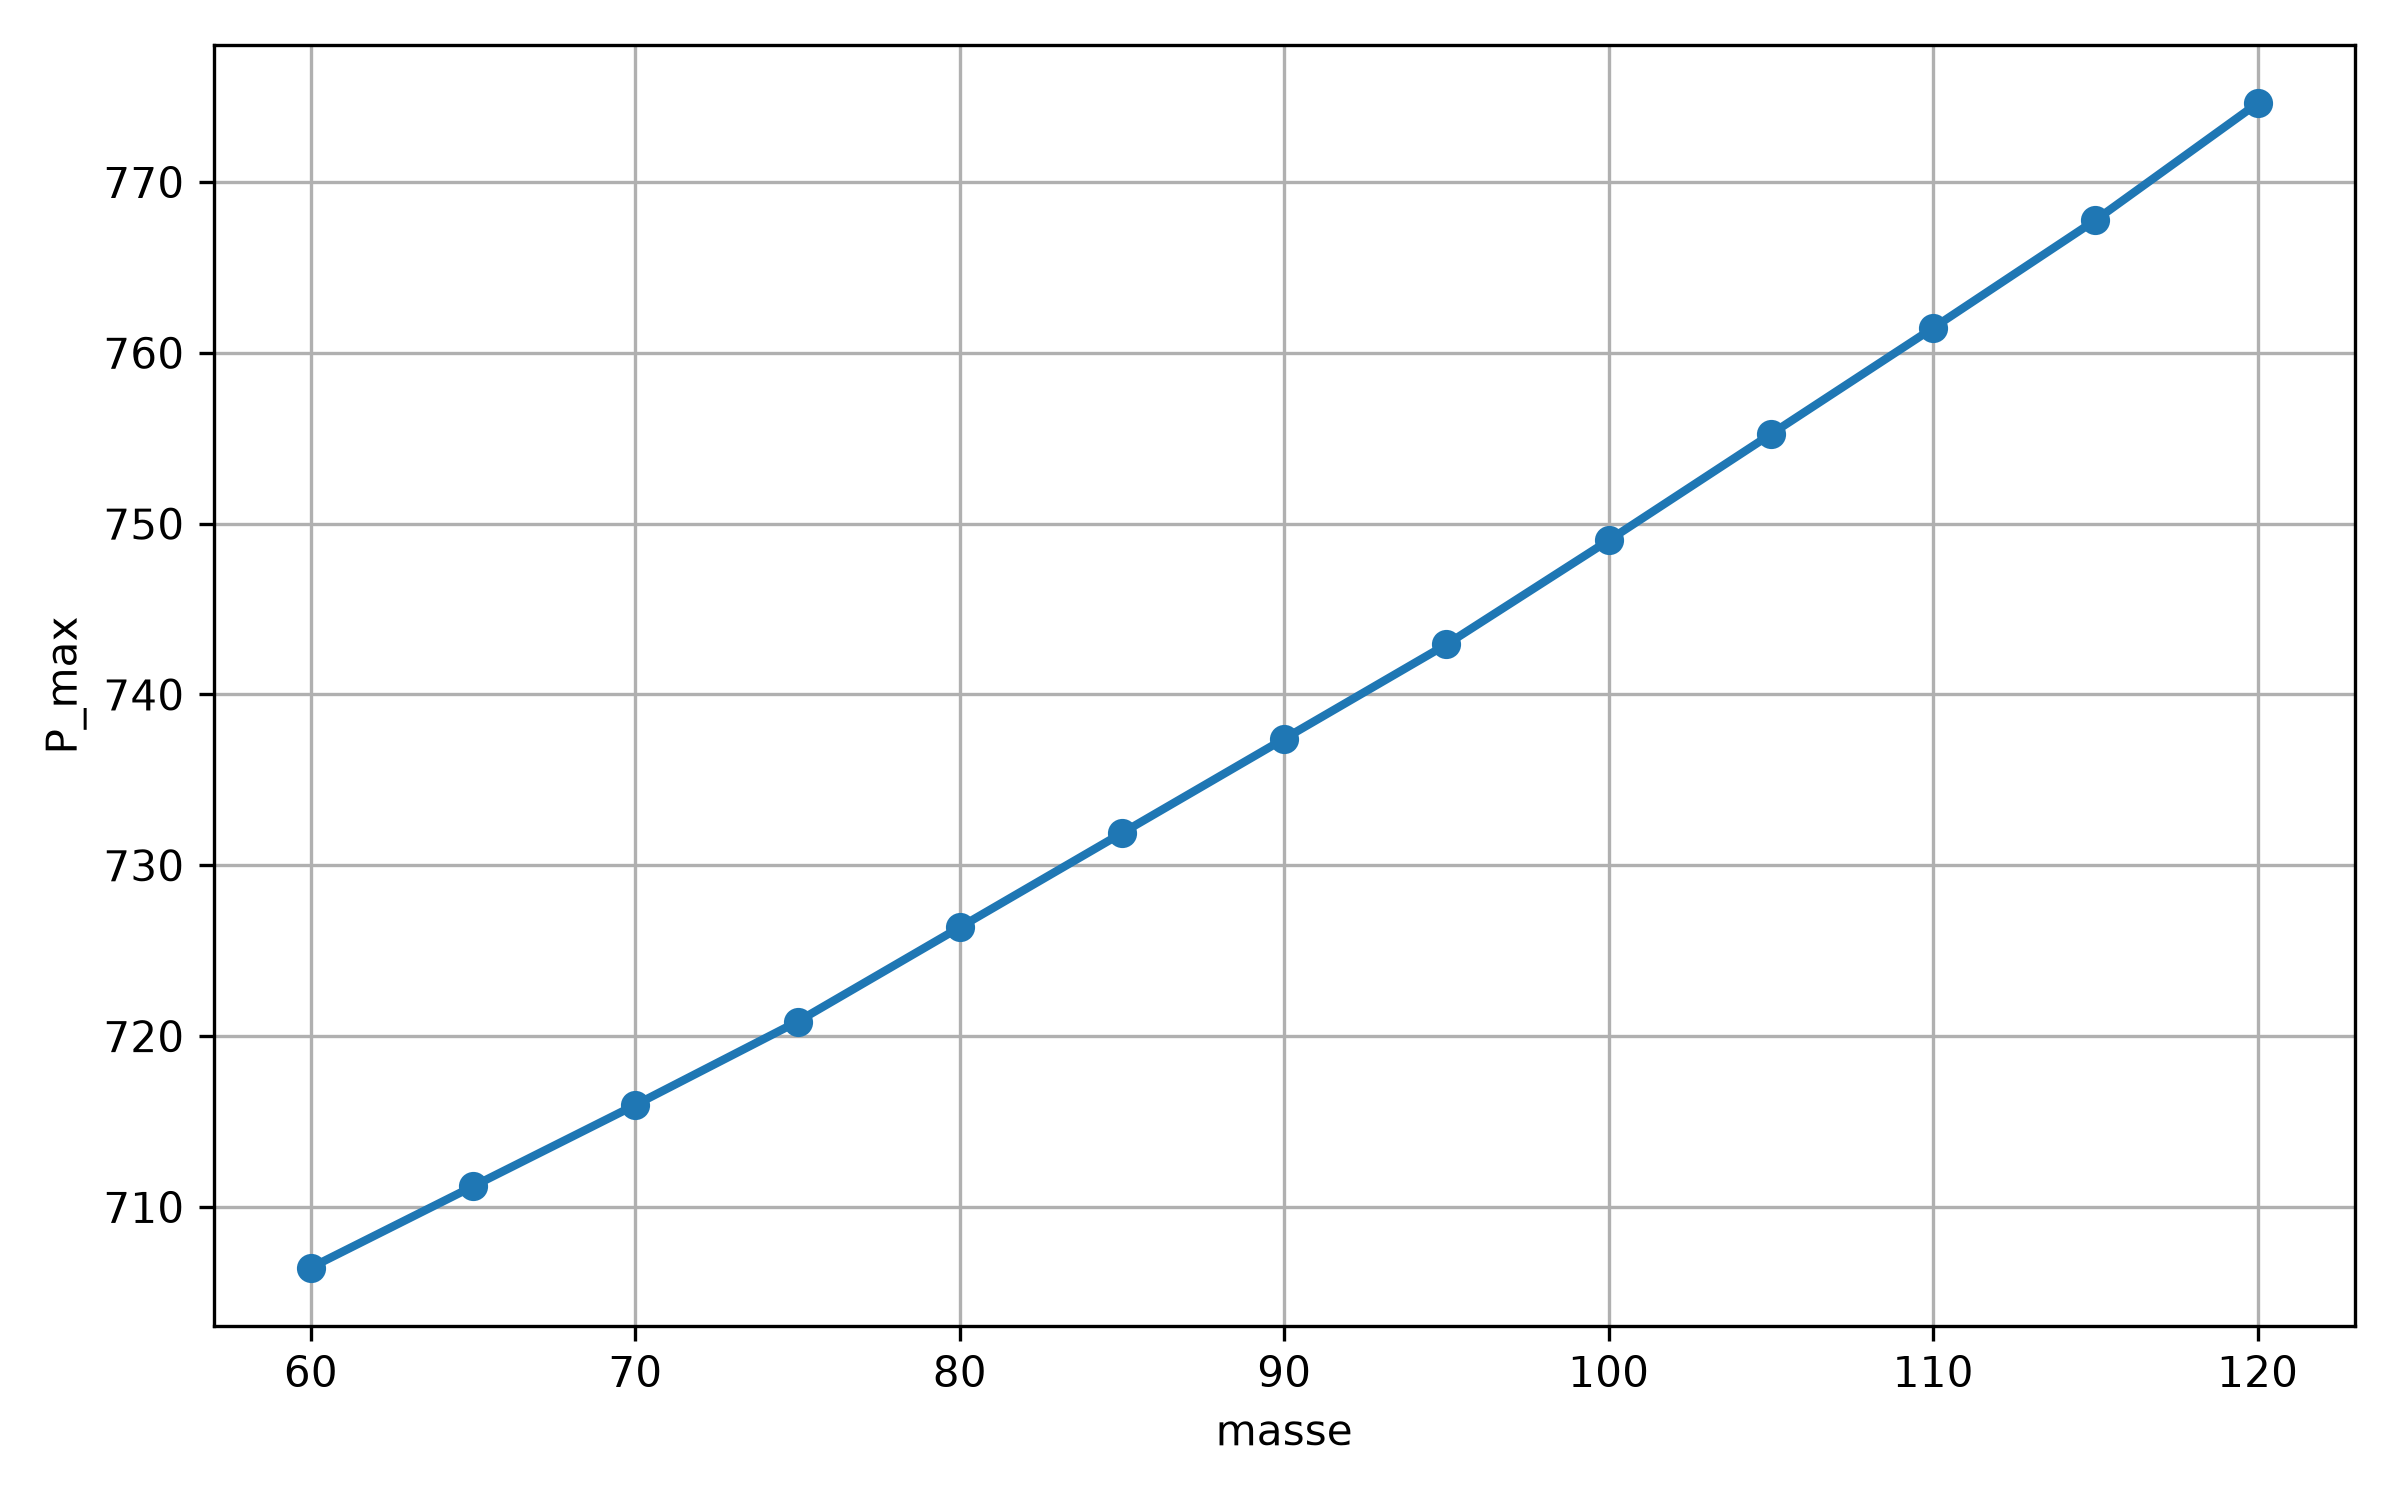
\includegraphics[width=0.95\textwidth]{Parameterstudie_masse_P_max.png}%
\caption{Parameterstudie\_masse\_P\_max}%
\end{figure}

%
\subsection{Parameterstudie\_r\_inch\_P\_max}%
\label{subsec:ParameterstudierinchPmax}%


\begin{figure}[H]%
\centering%
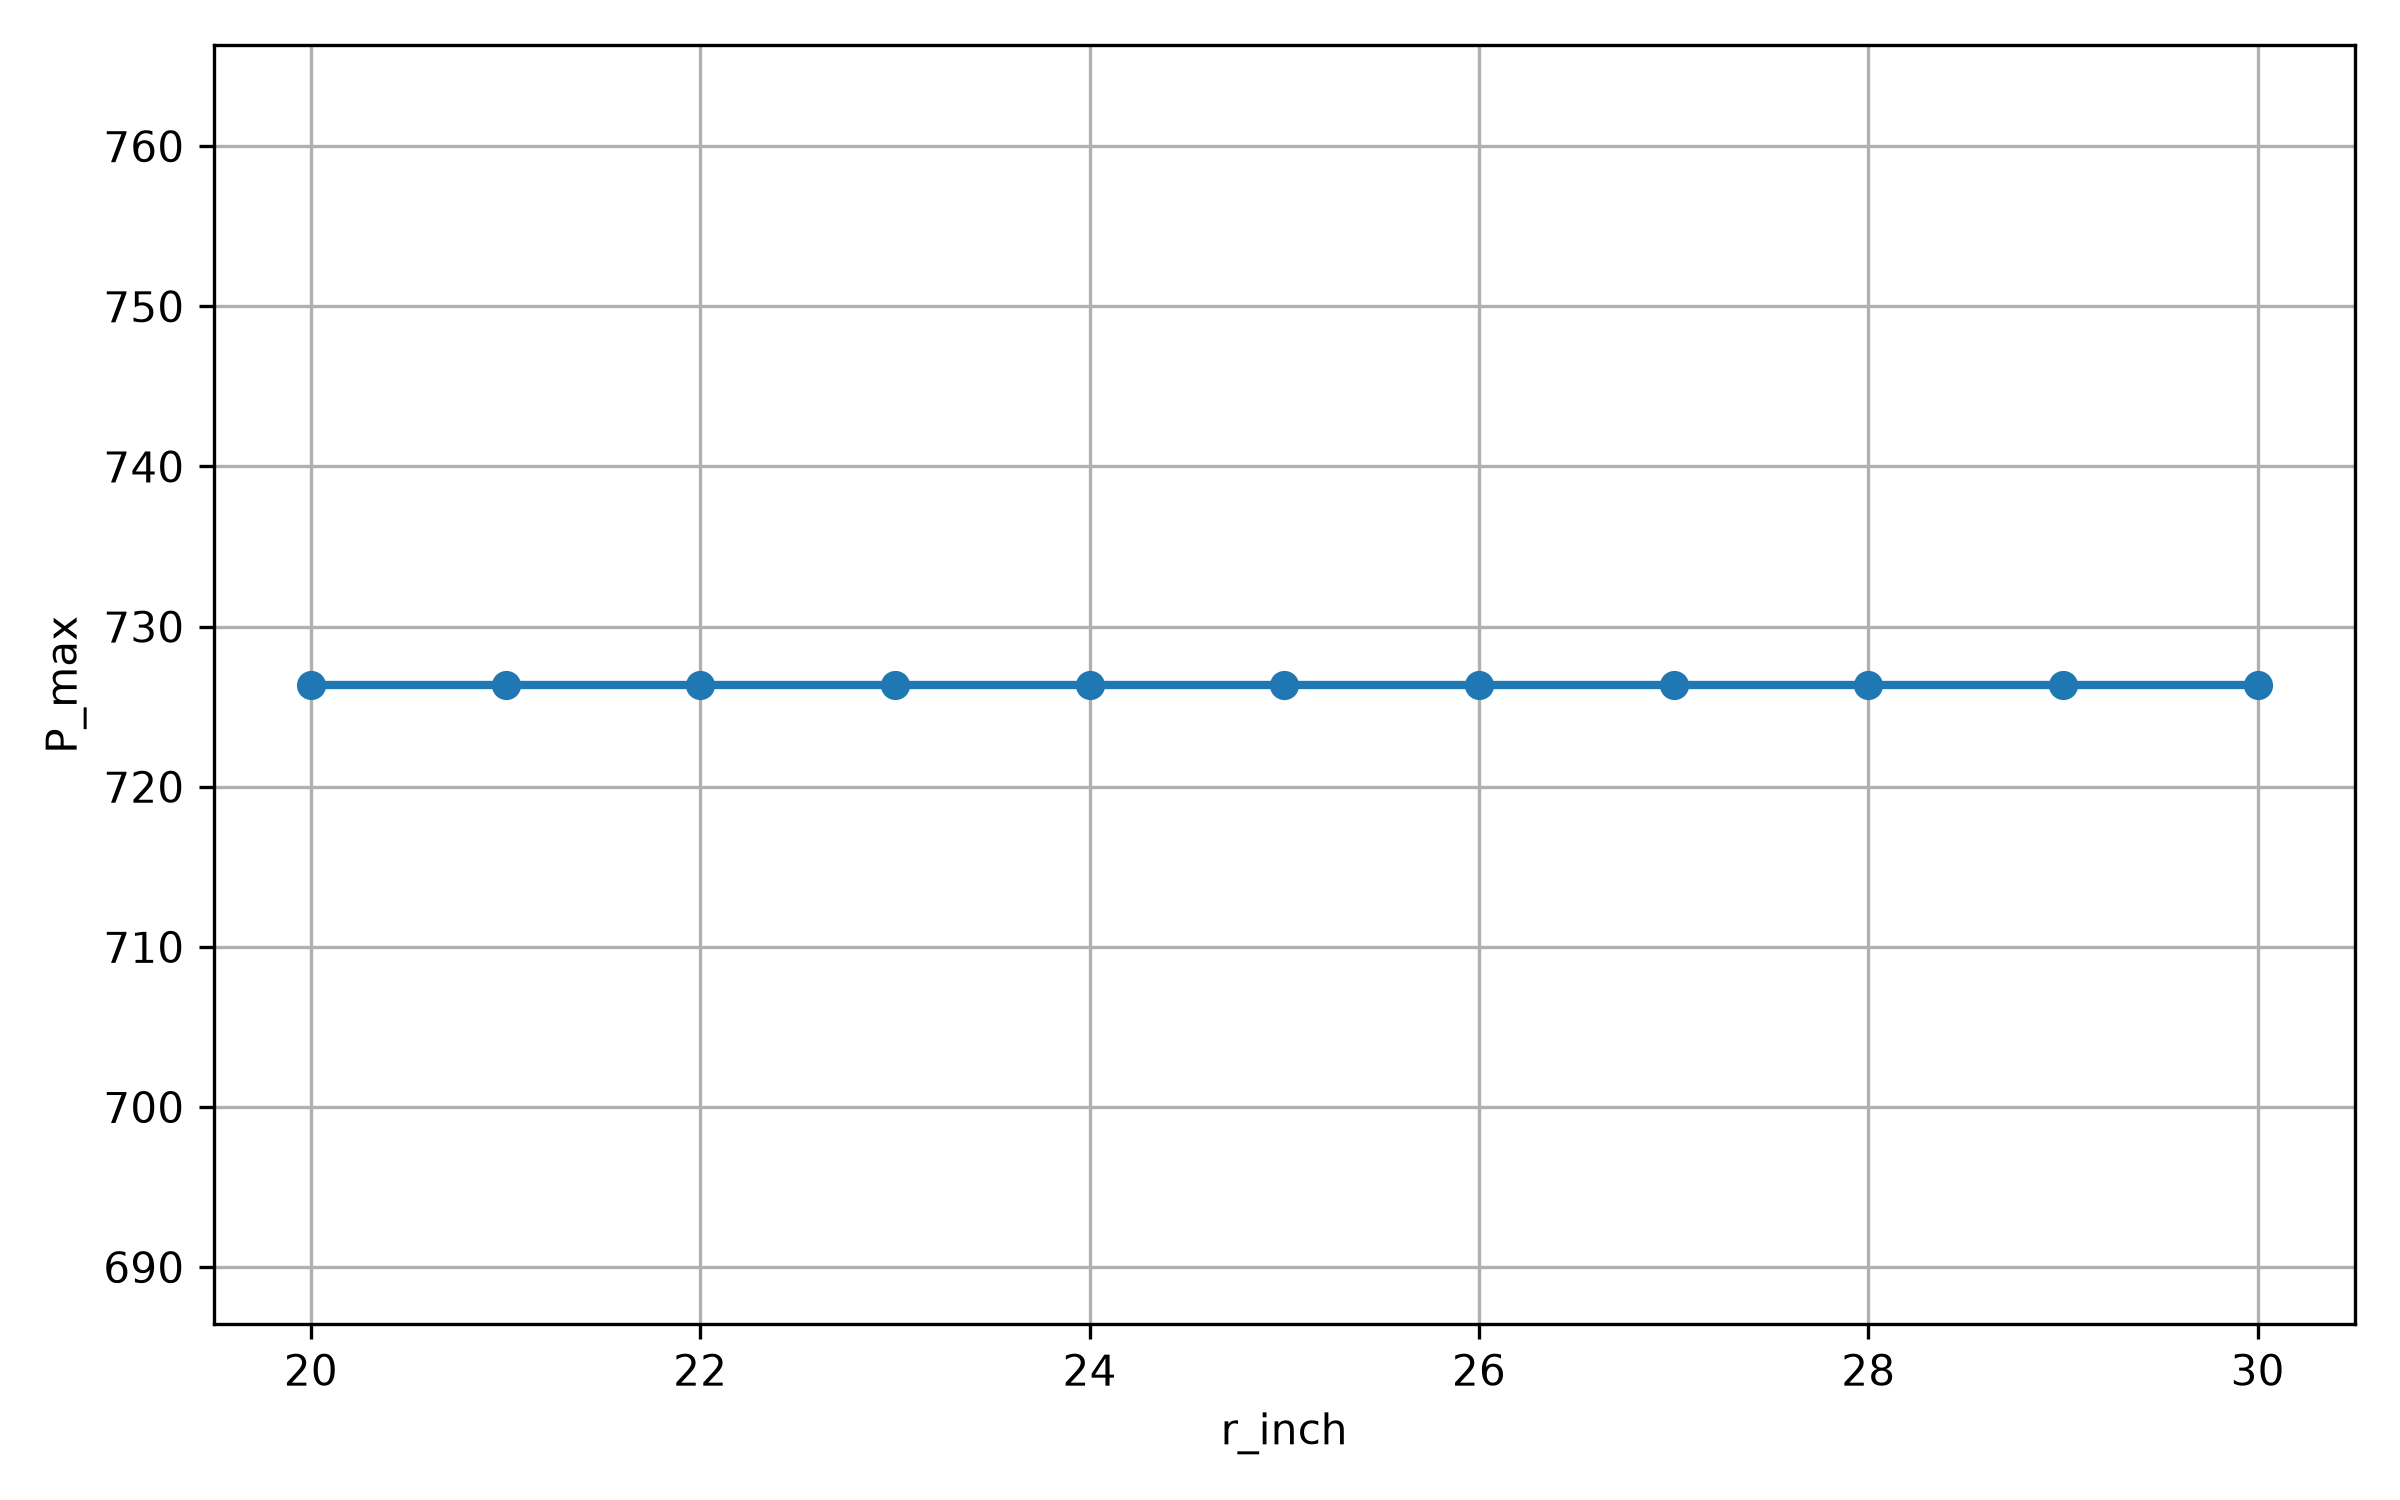
\includegraphics[width=0.95\textwidth]{Parameterstudie_r_inch_P_max.png}%
\caption{Parameterstudie\_r\_inch\_P\_max}%
\end{figure}

%
\subsection{SOC}%
\label{subsec:SOC}%


\begin{figure}[H]%
\centering%
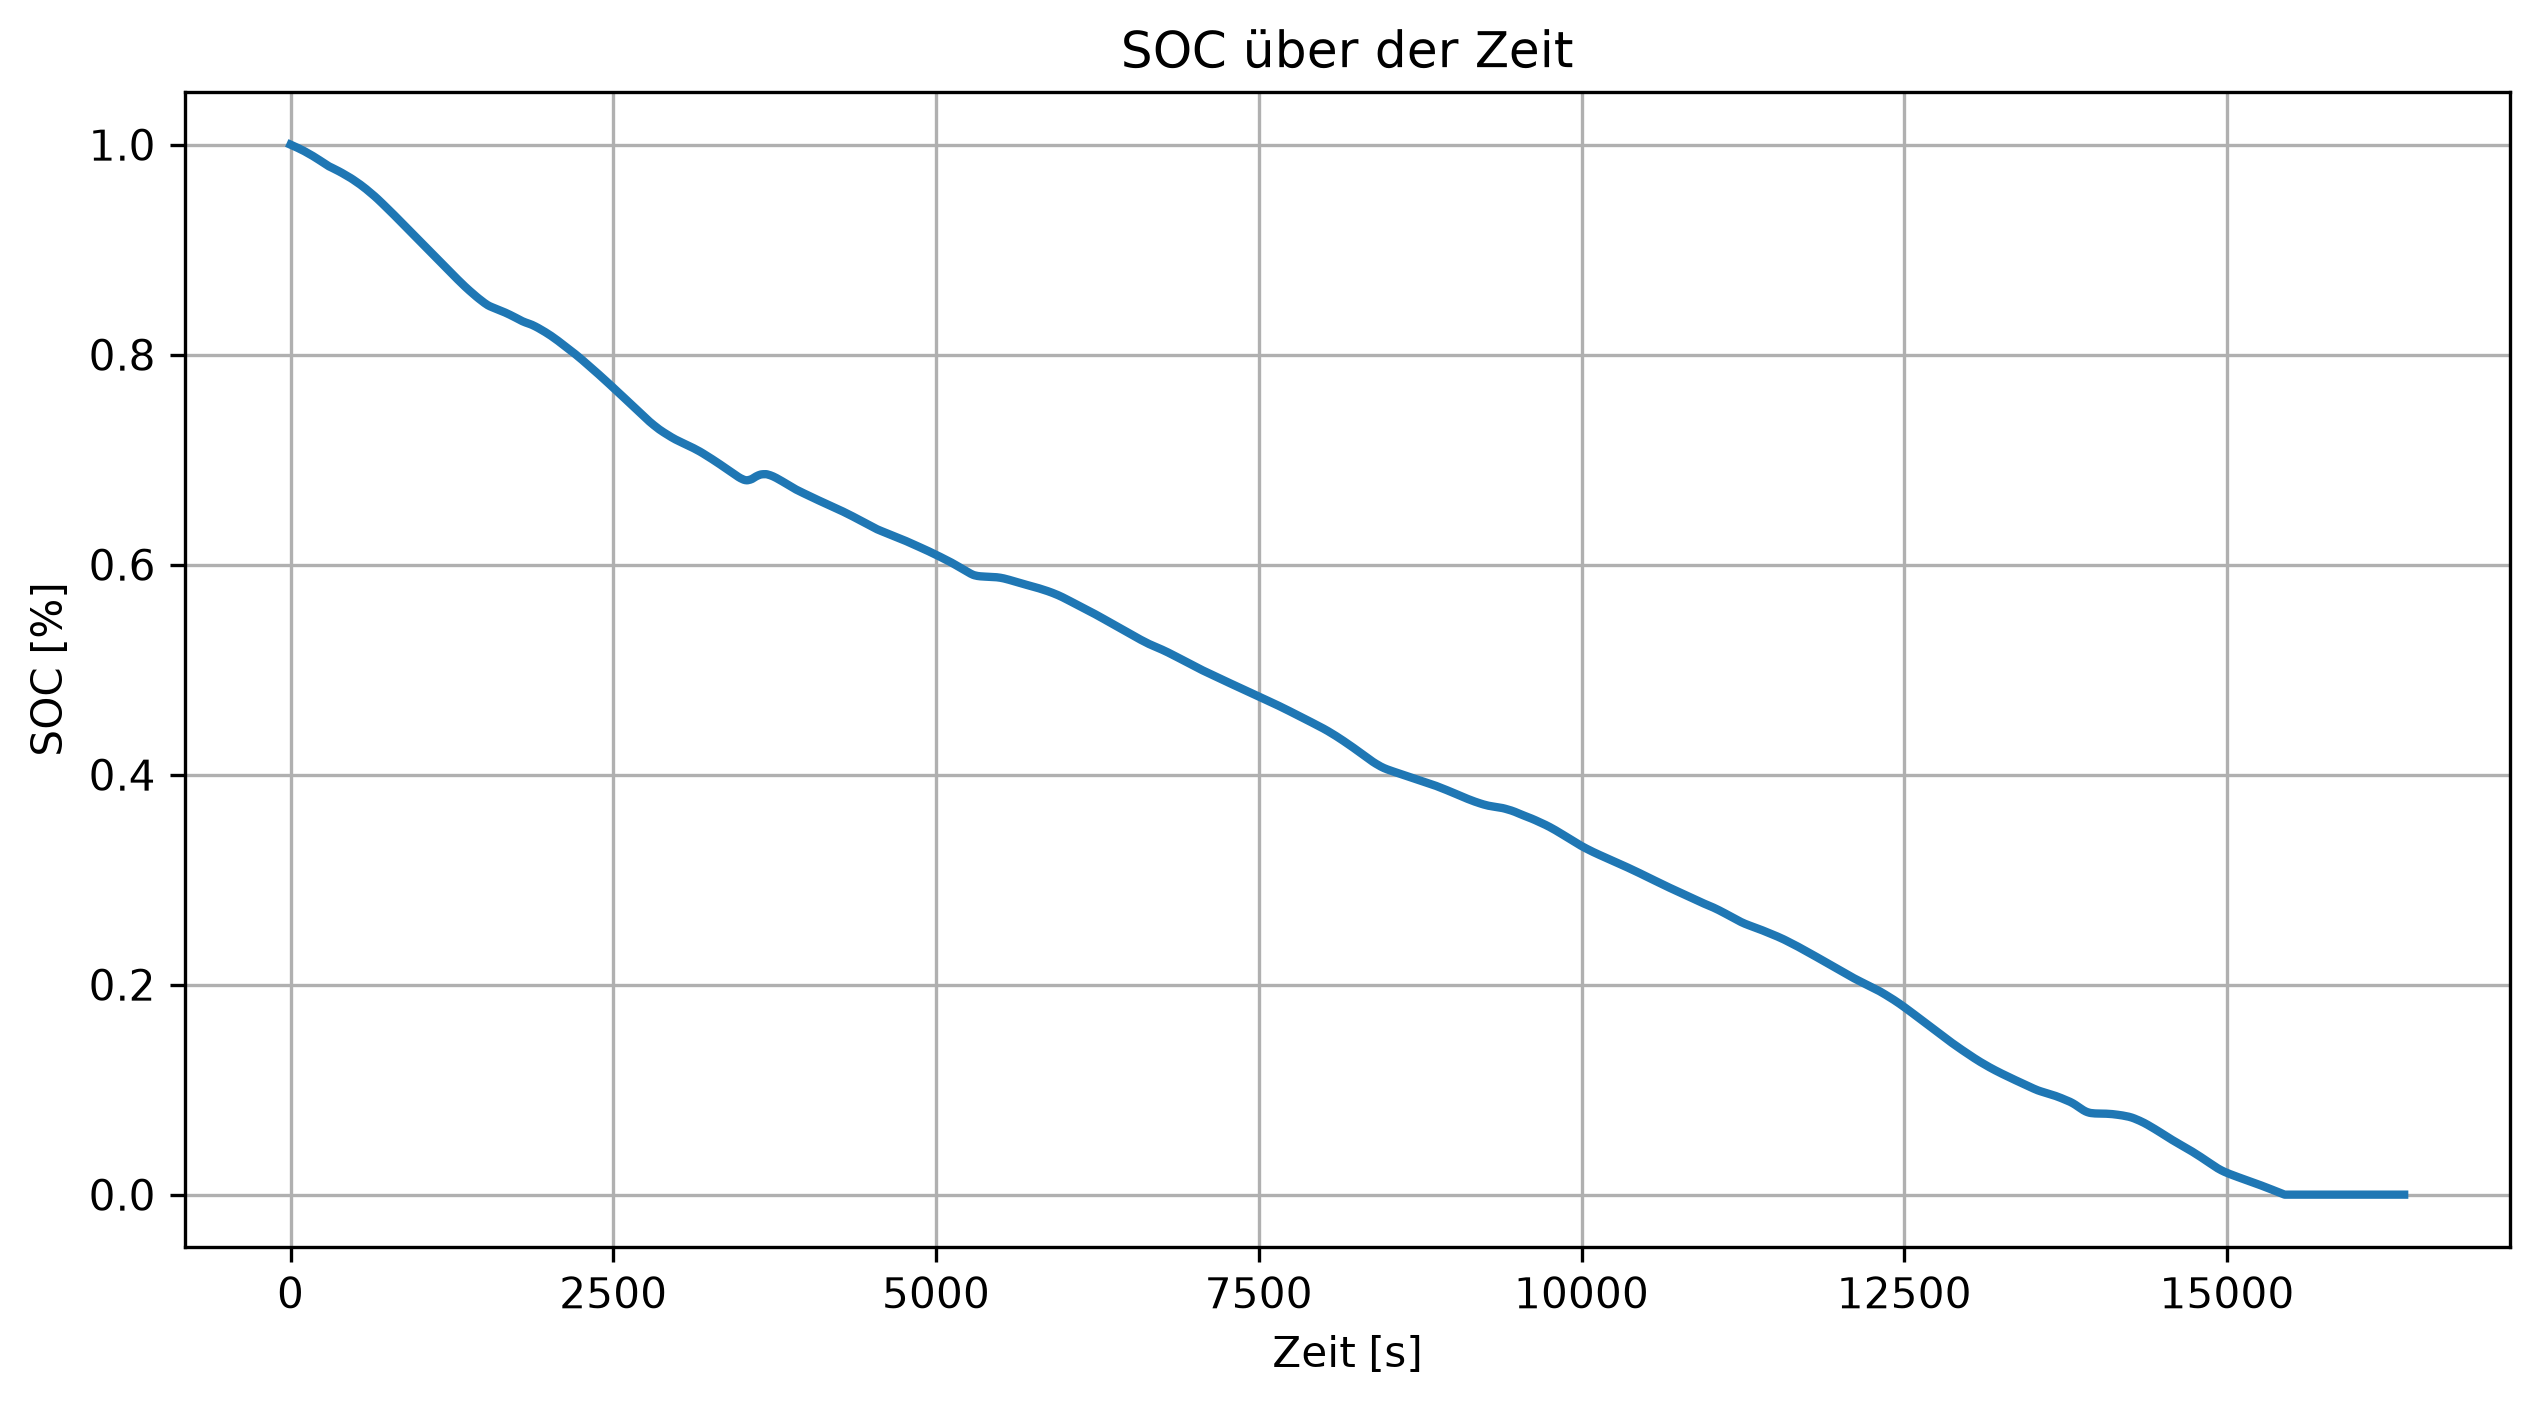
\includegraphics[width=0.95\textwidth]{SOC.png}%
\caption{SOC}%
\end{figure}

%
\subsection{T\_drehmoment}%
\label{subsec:Tdrehmoment}%


\begin{figure}[H]%
\centering%
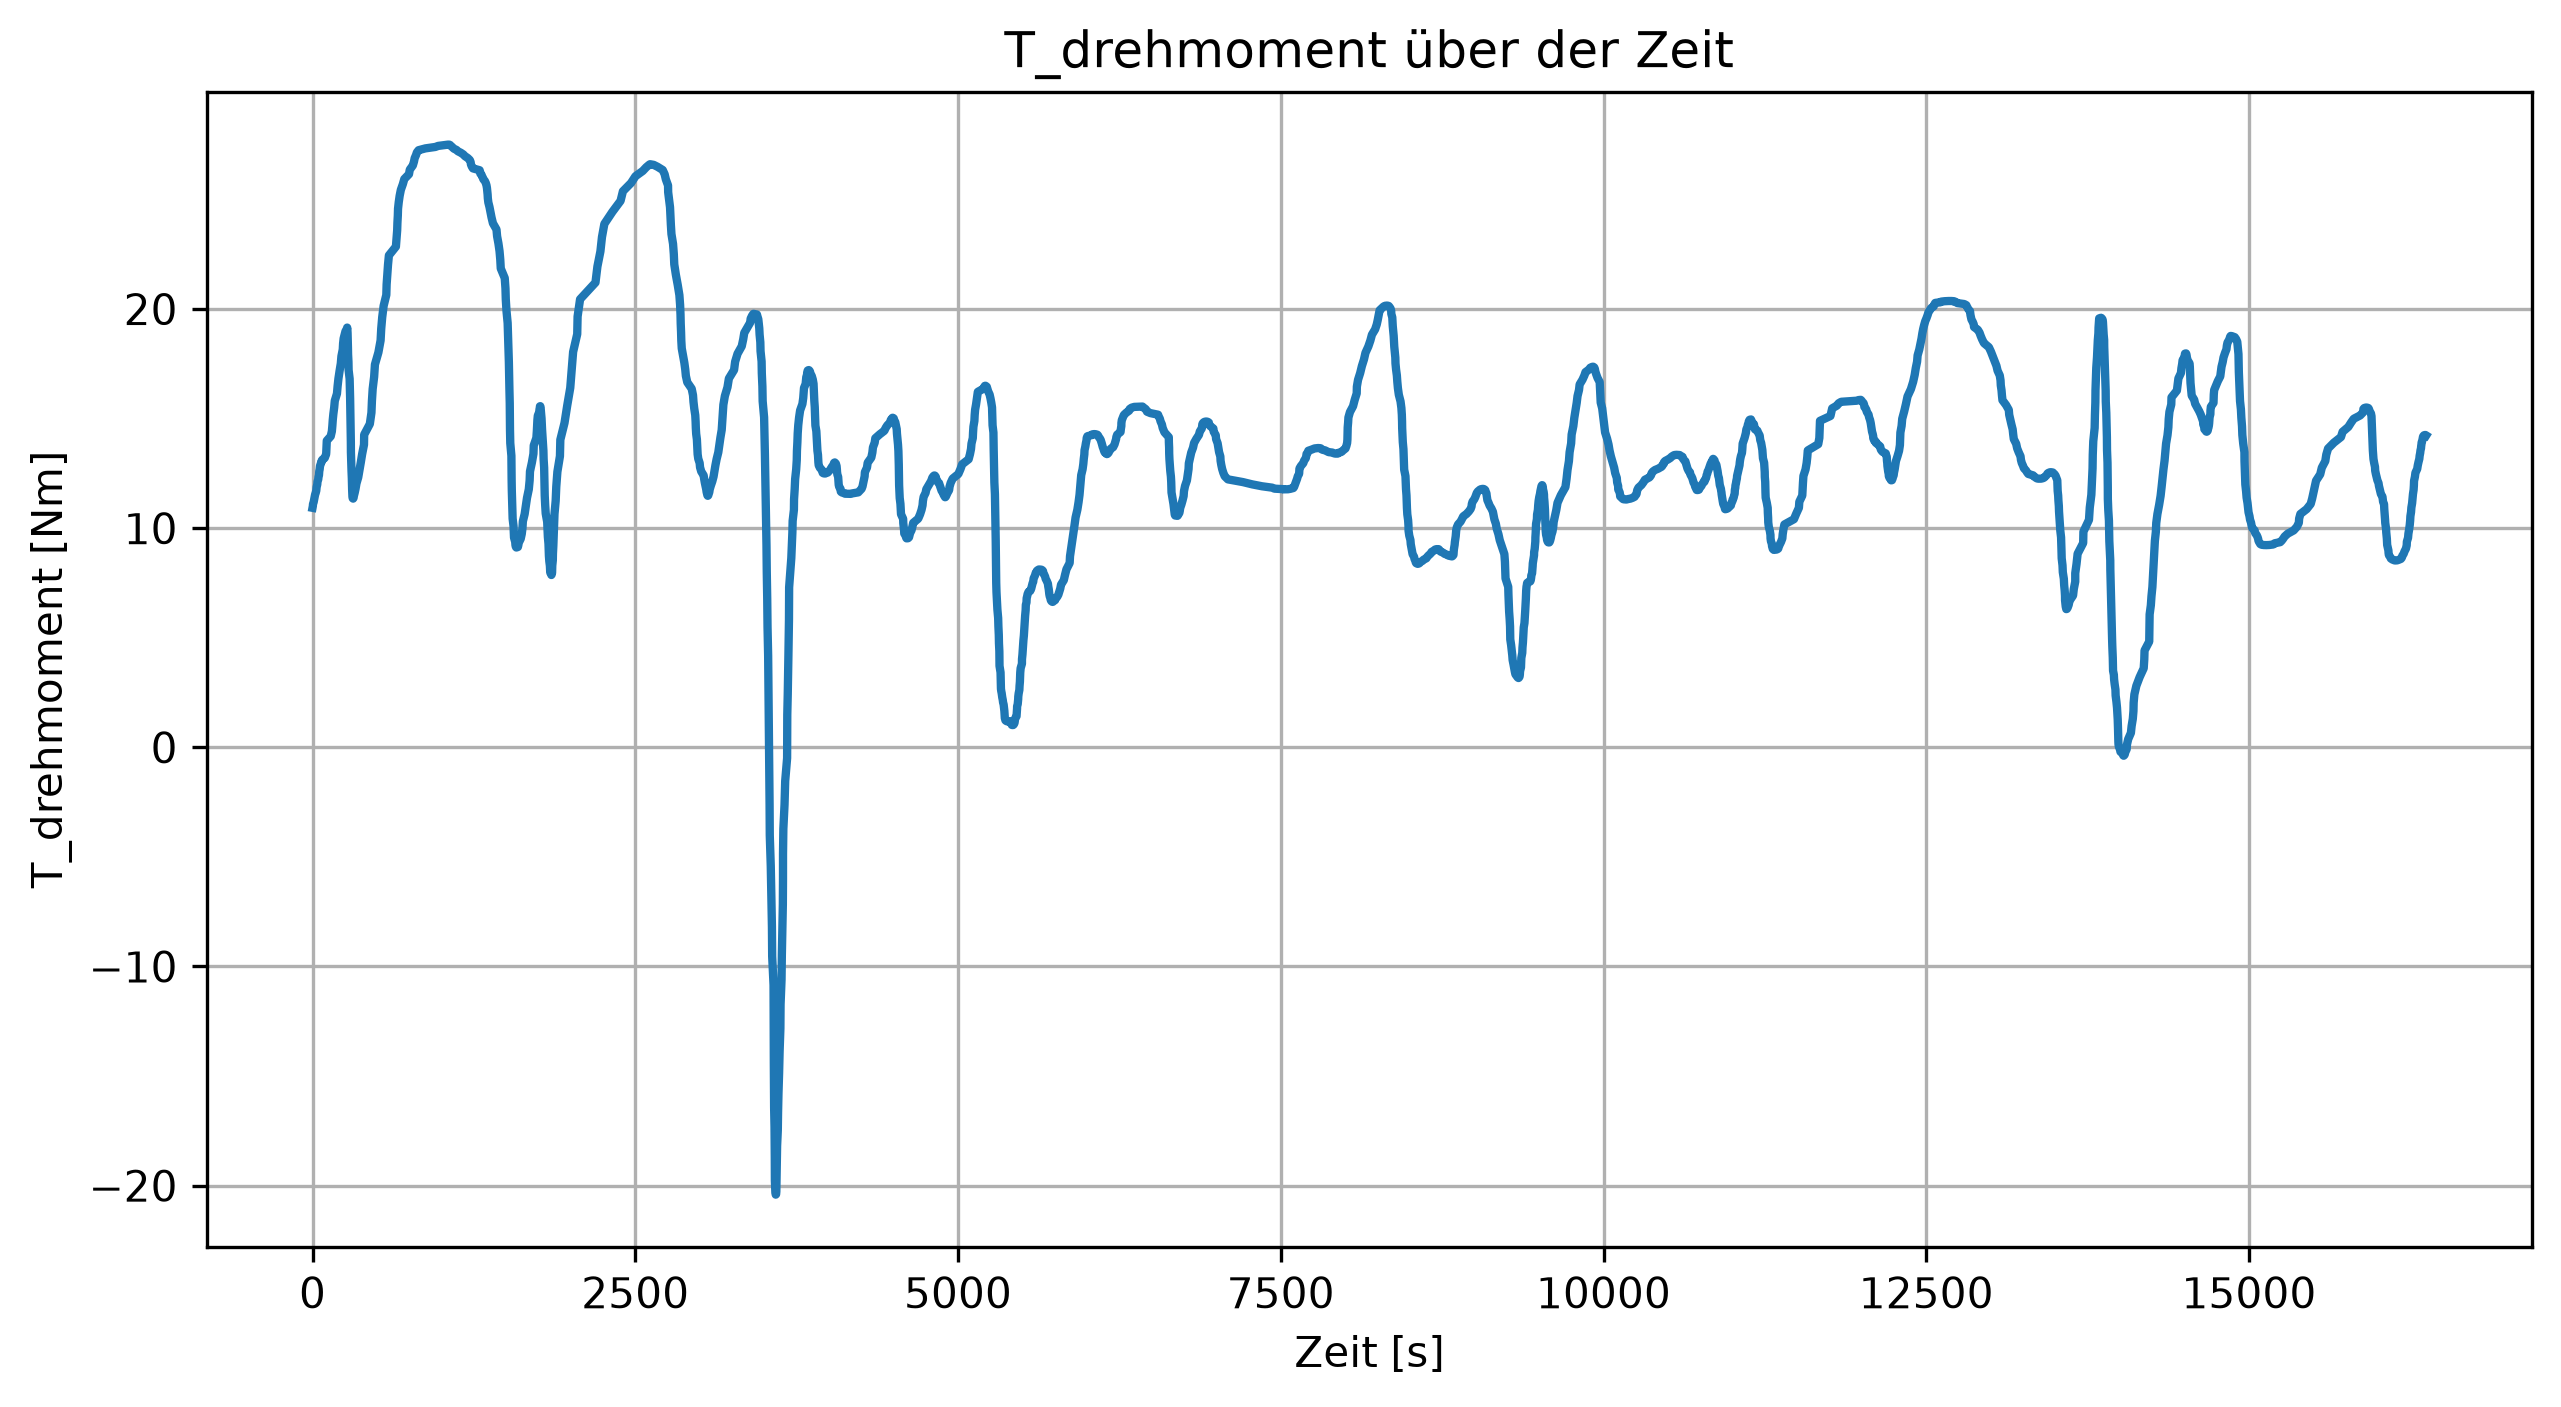
\includegraphics[width=0.95\textwidth]{T_drehmoment.png}%
\caption{T\_drehmoment}%
\end{figure}

%
\subsection{a}%
\label{subsec:a}%


\begin{figure}[H]%
\centering%
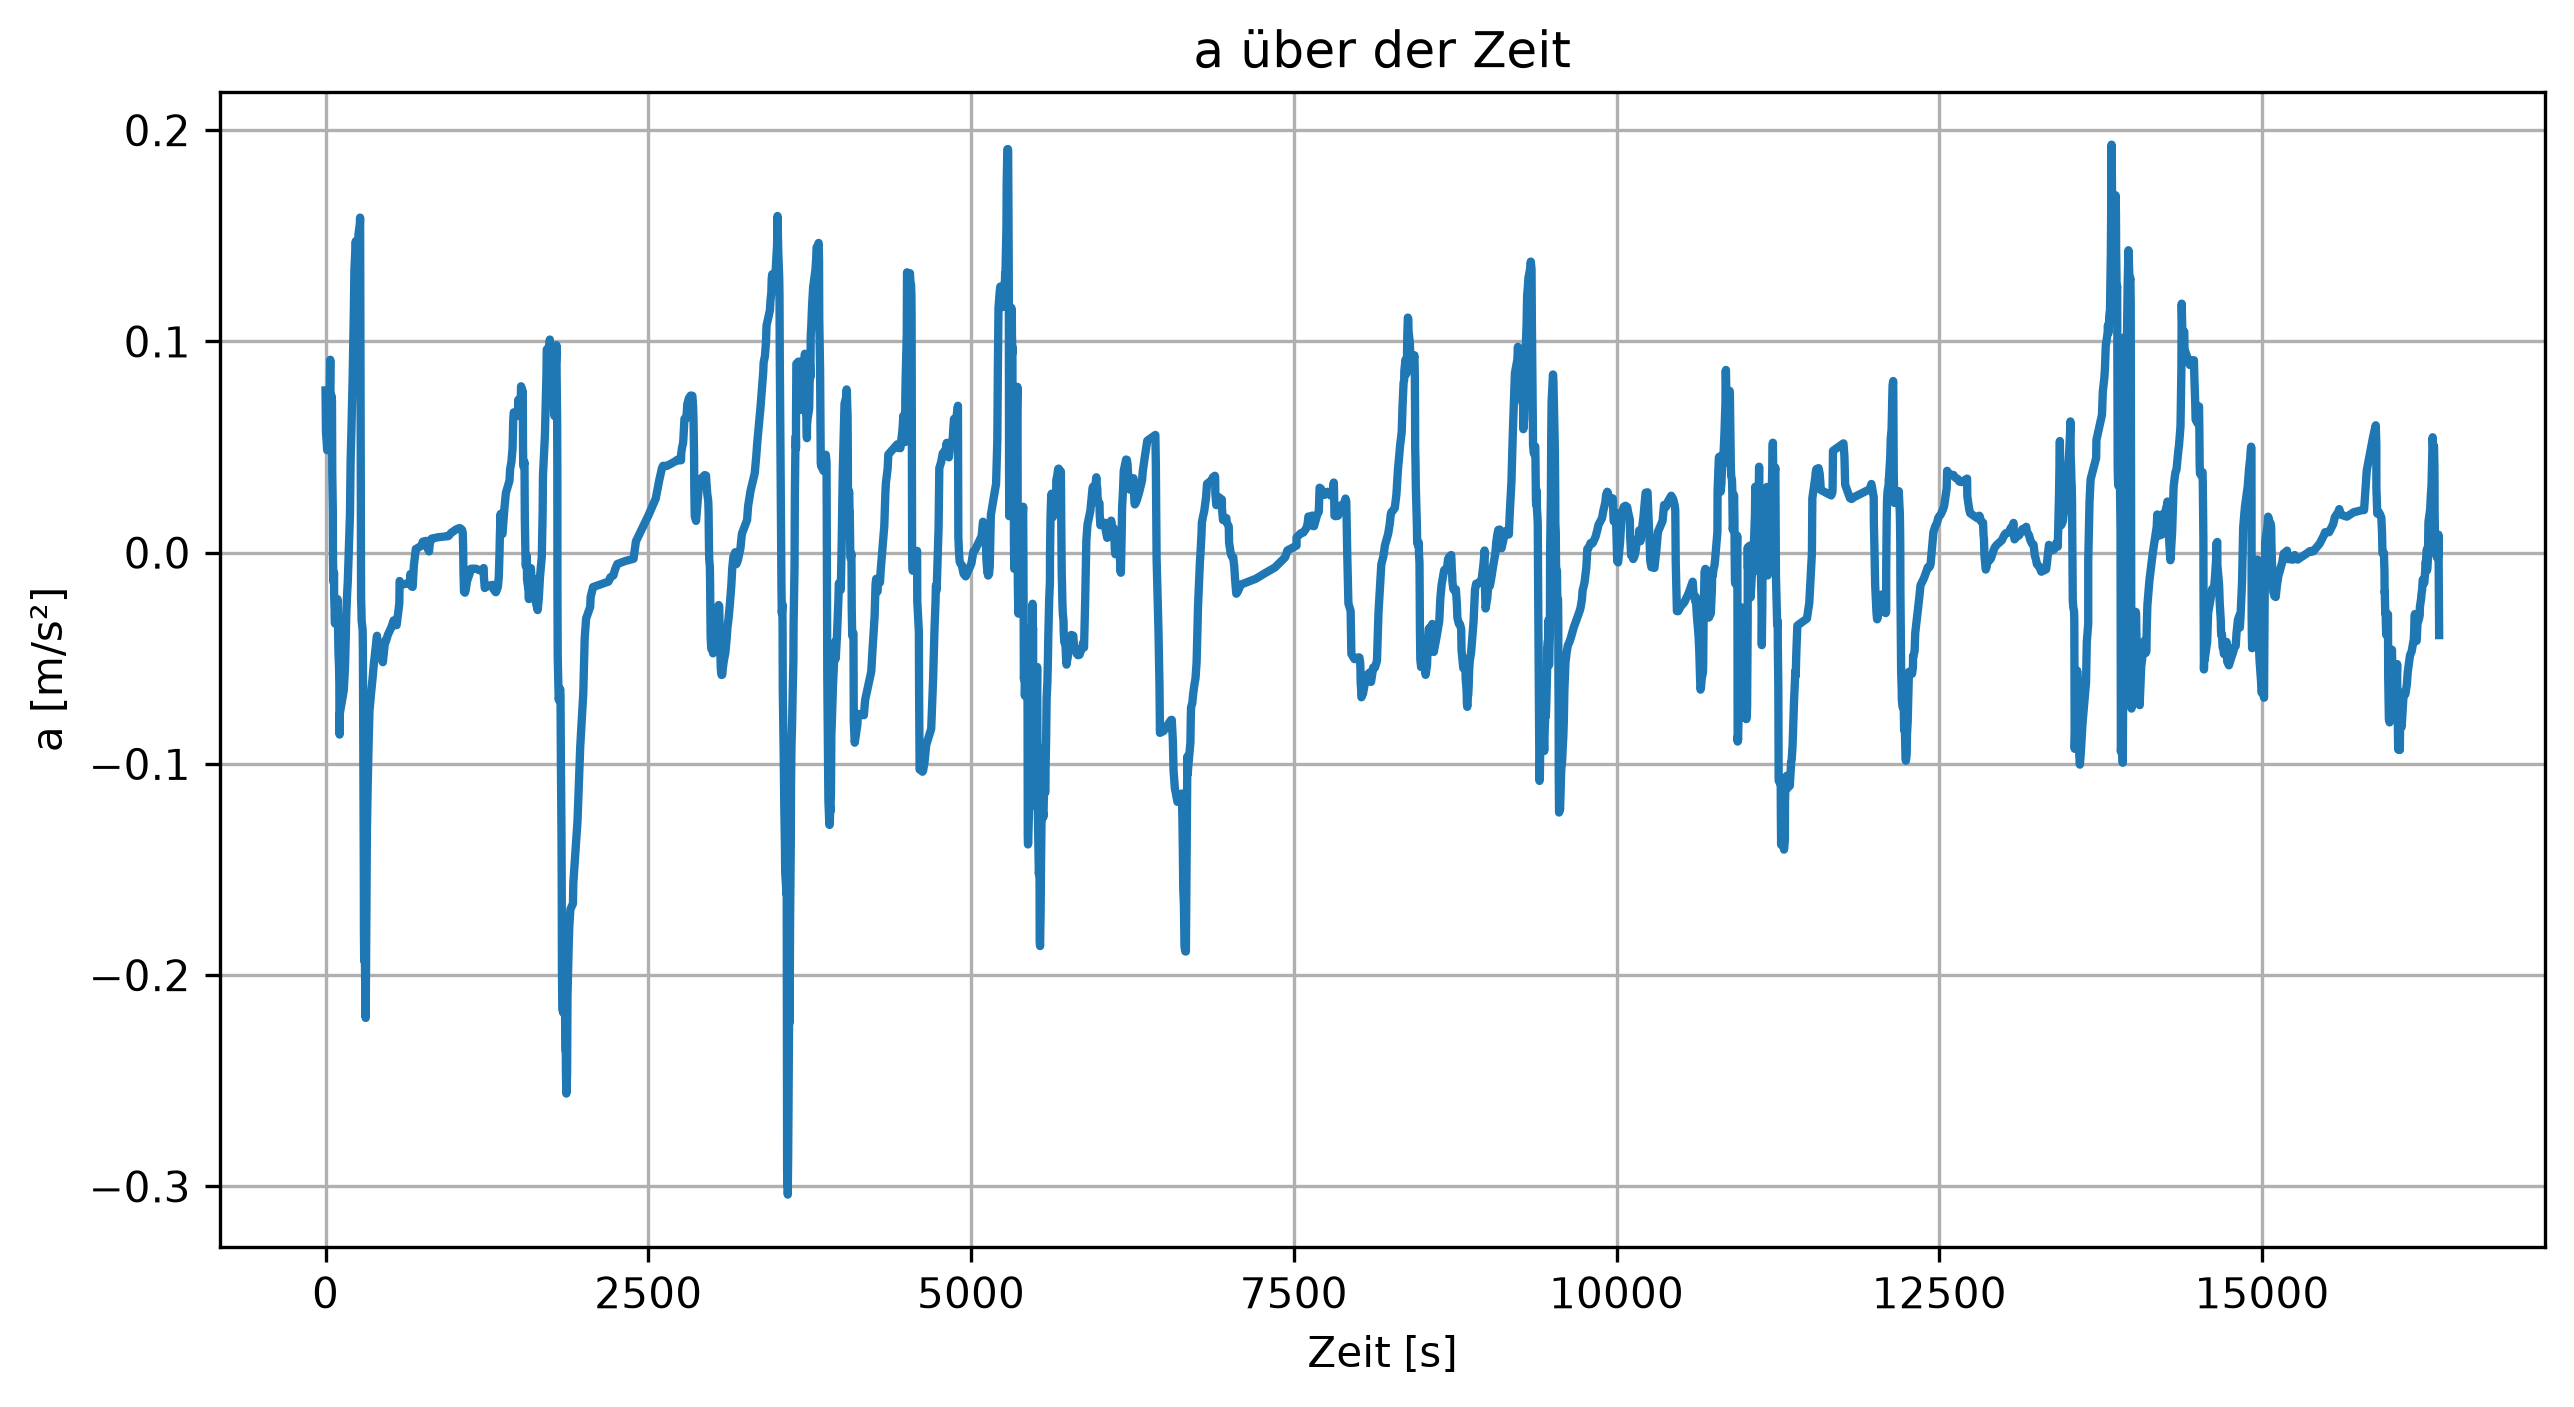
\includegraphics[width=0.95\textwidth]{a.png}%
\caption{a}%
\end{figure}

%
\subsection{bearing}%
\label{subsec:bearing}%


\begin{figure}[H]%
\centering%
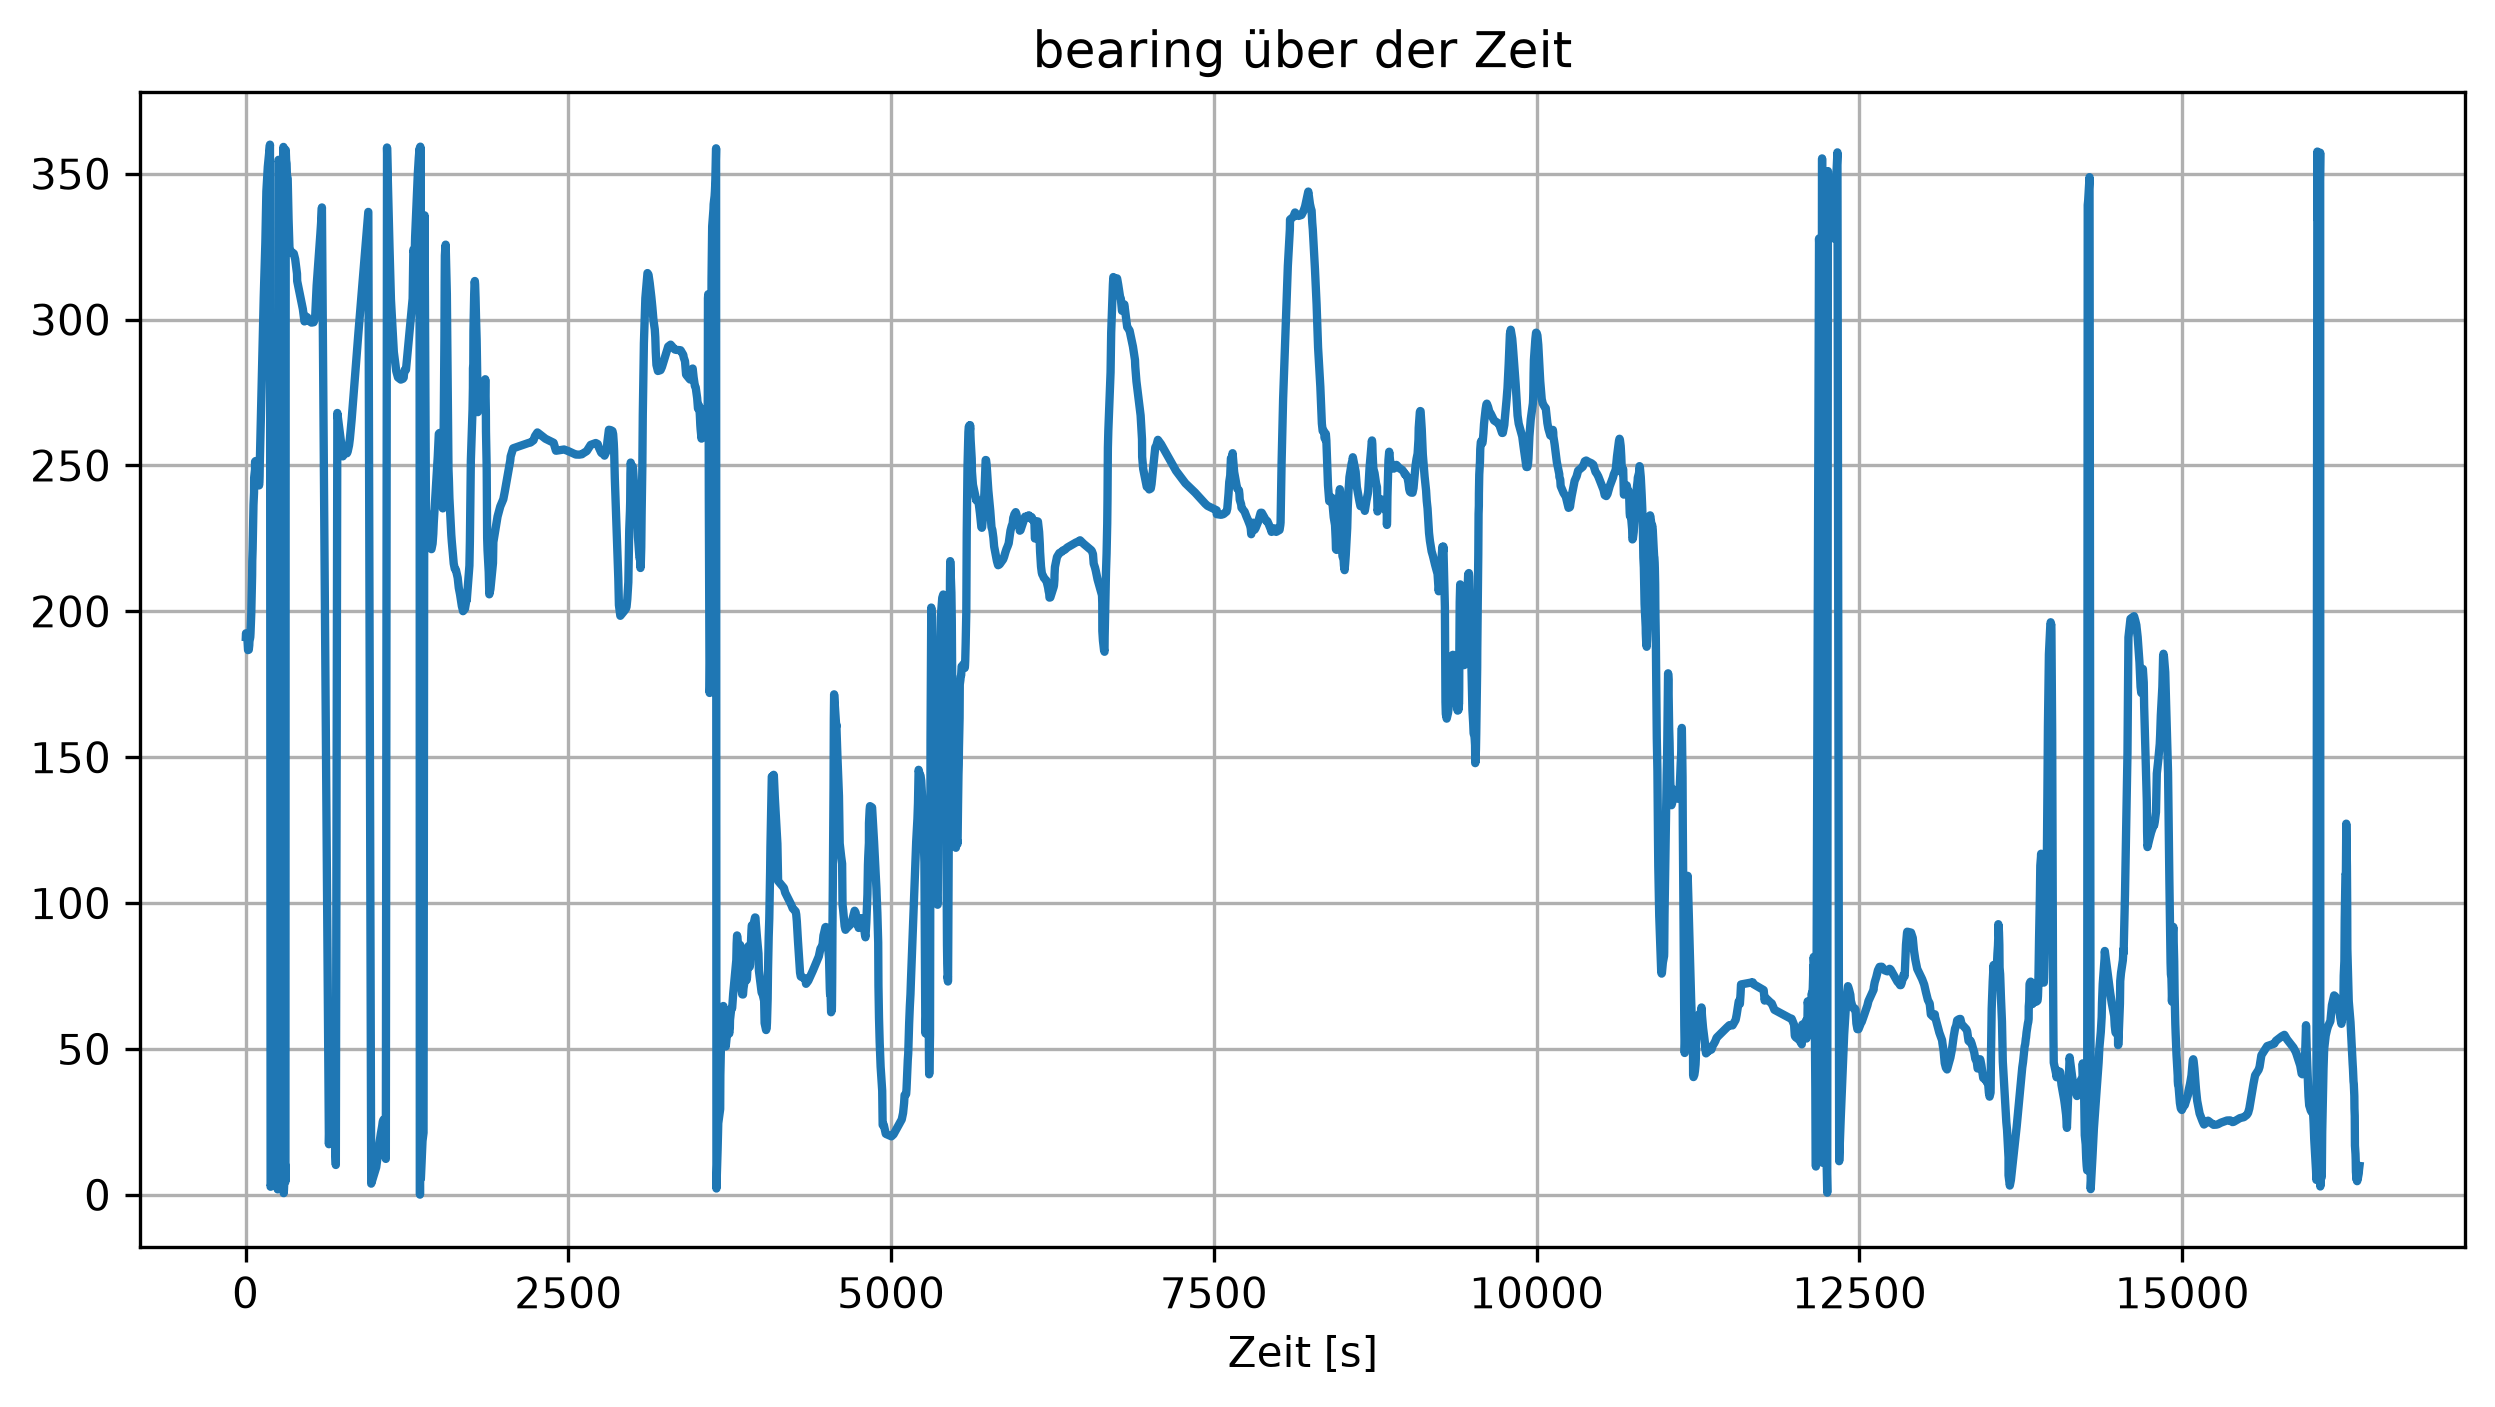
\includegraphics[width=0.95\textwidth]{bearing.png}%
\caption{bearing}%
\end{figure}

%
\subsection{ds\_orig}%
\label{subsec:dsorig}%


\begin{figure}[H]%
\centering%
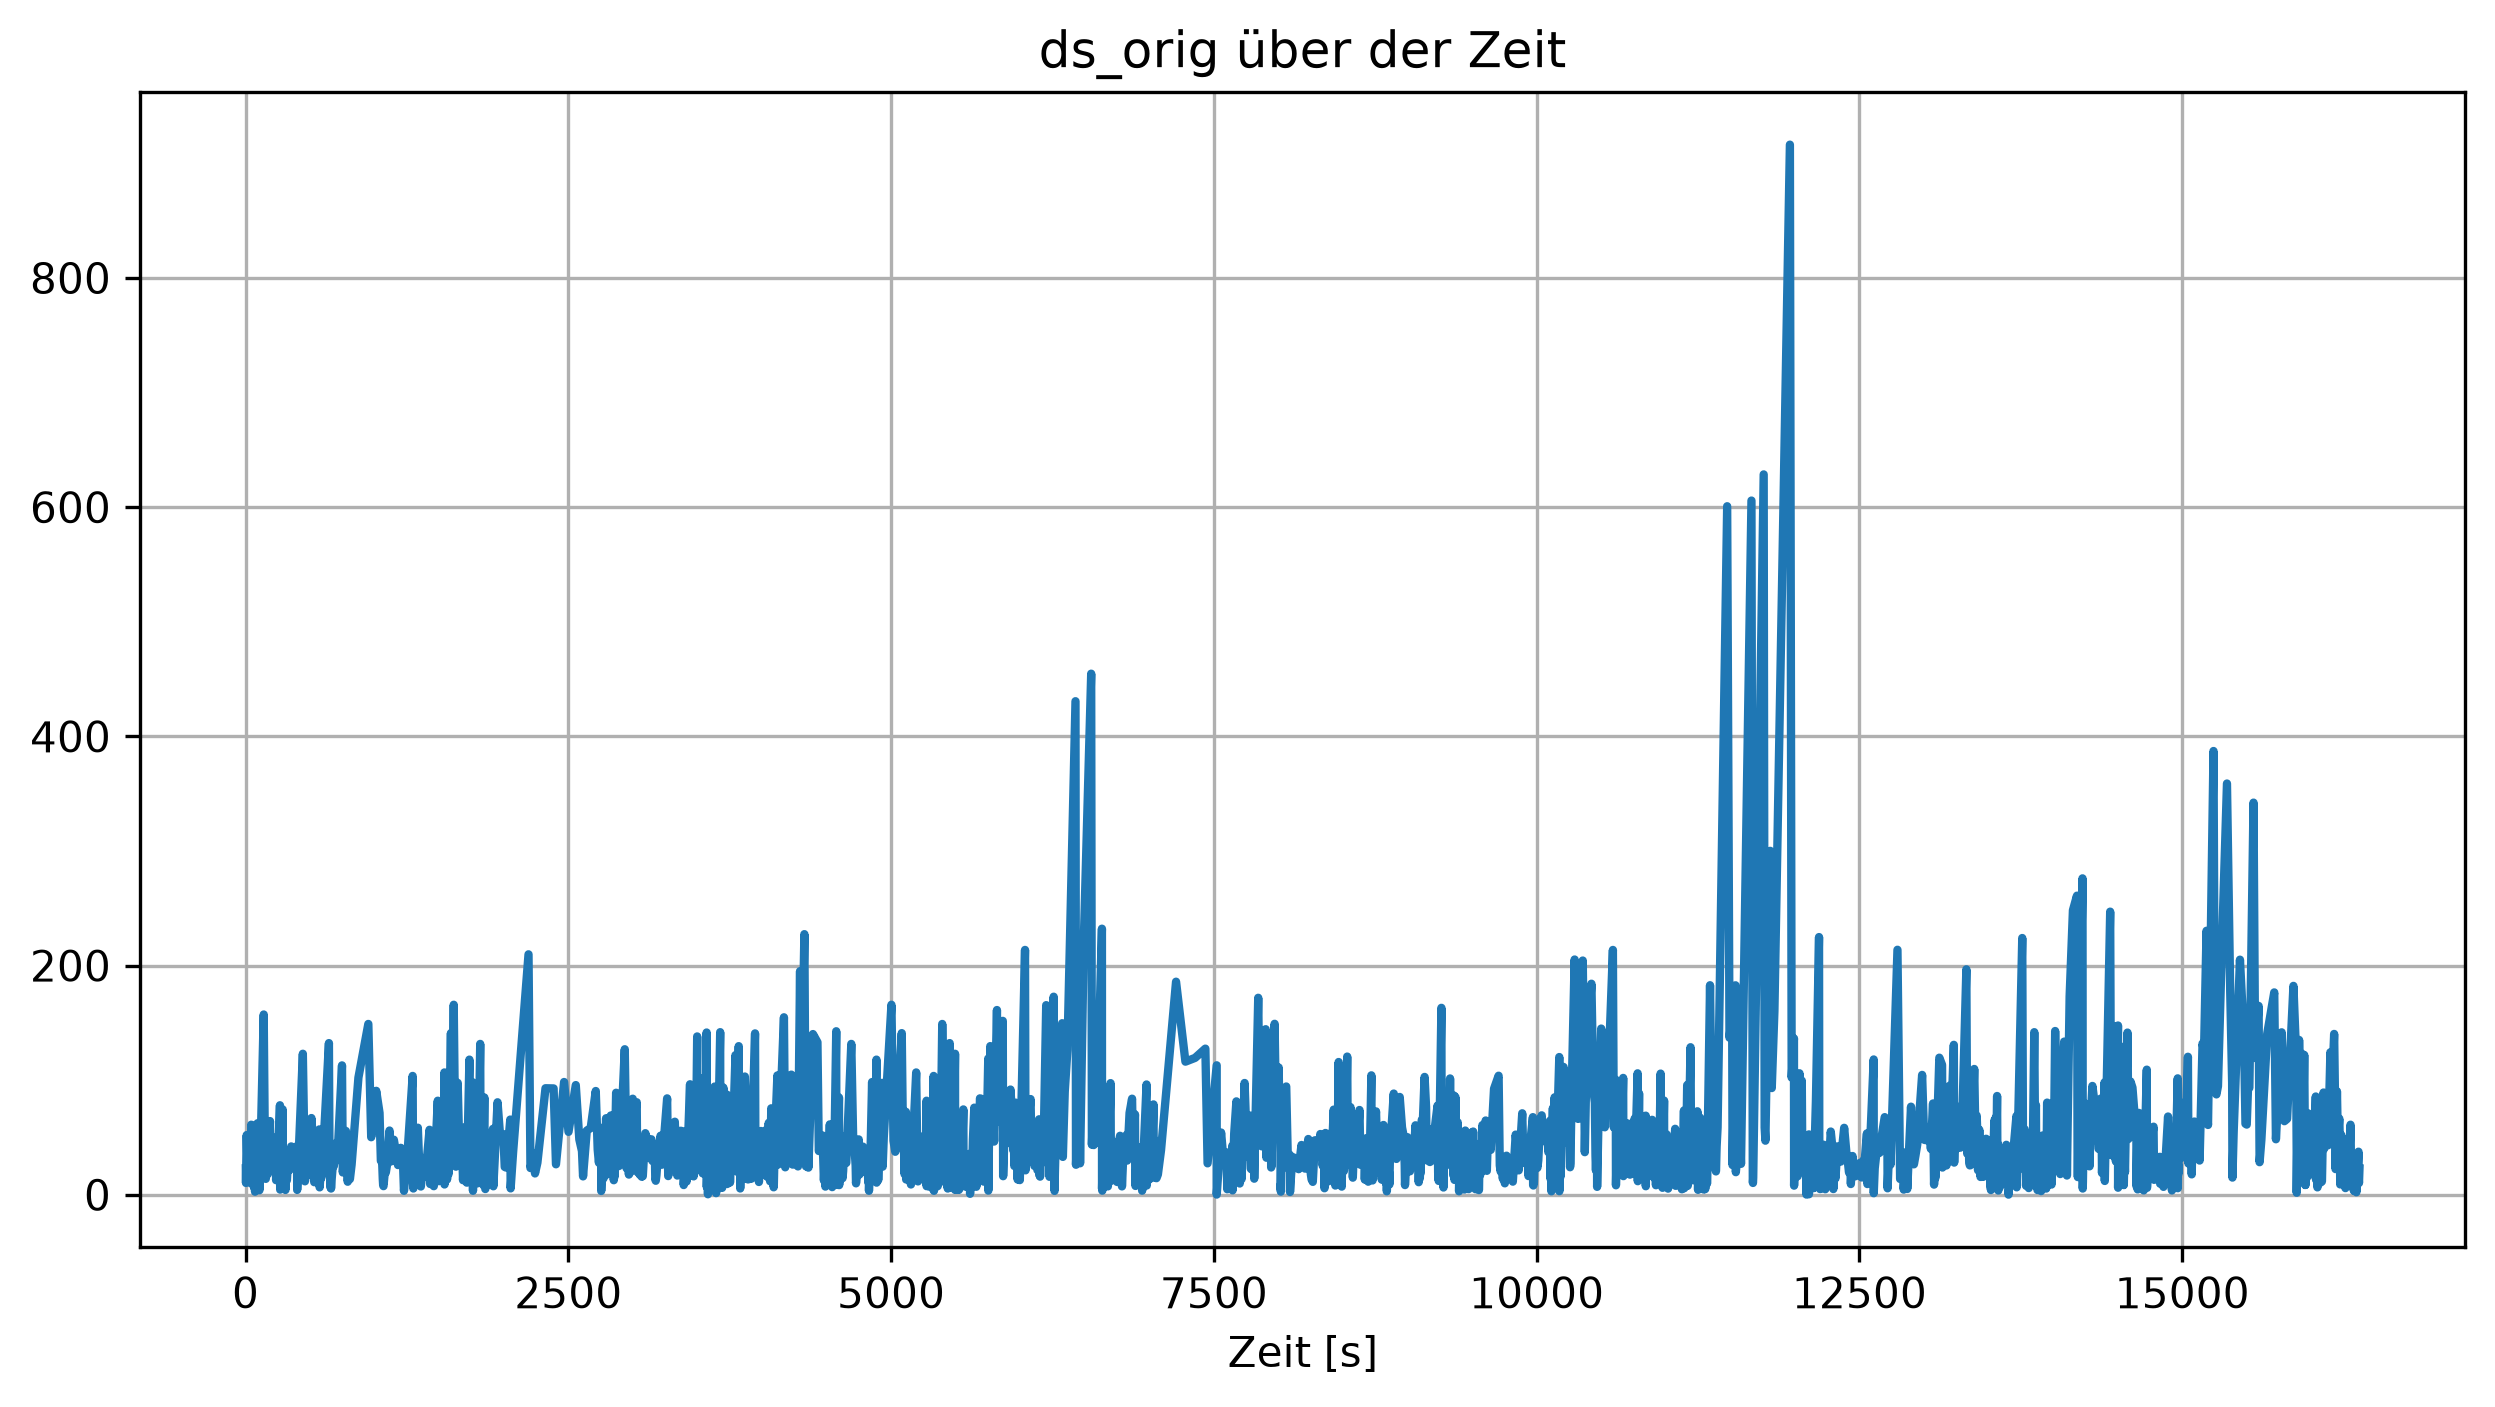
\includegraphics[width=0.95\textwidth]{ds_orig.png}%
\caption{ds\_orig}%
\end{figure}

%
\subsection{hoehenprofil\_steigung}%
\label{subsec:hoehenprofilsteigung}%


\begin{figure}[H]%
\centering%
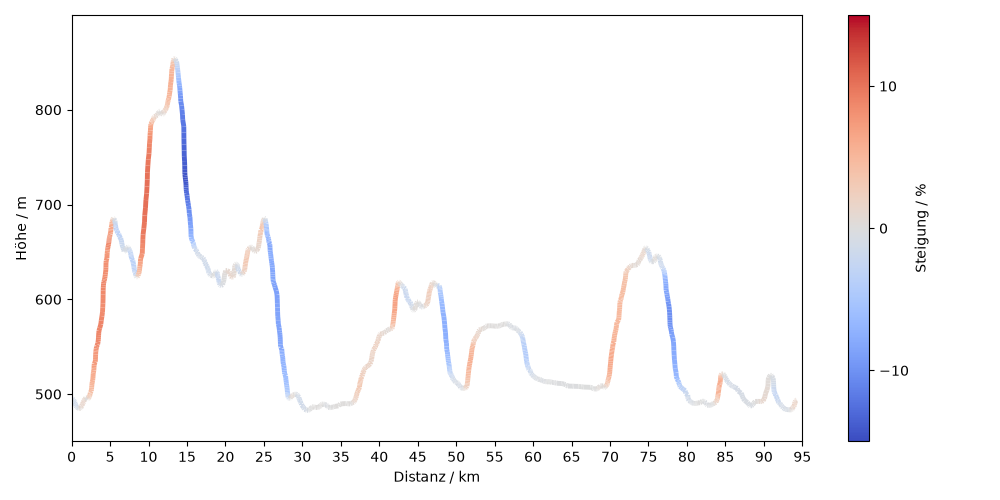
\includegraphics[width=0.95\textwidth]{hoehenprofil_steigung.png}%
\caption{hoehenprofil\_steigung}%
\end{figure}

%
\subsection{phi\_grad}%
\label{subsec:phigrad}%


\begin{figure}[H]%
\centering%
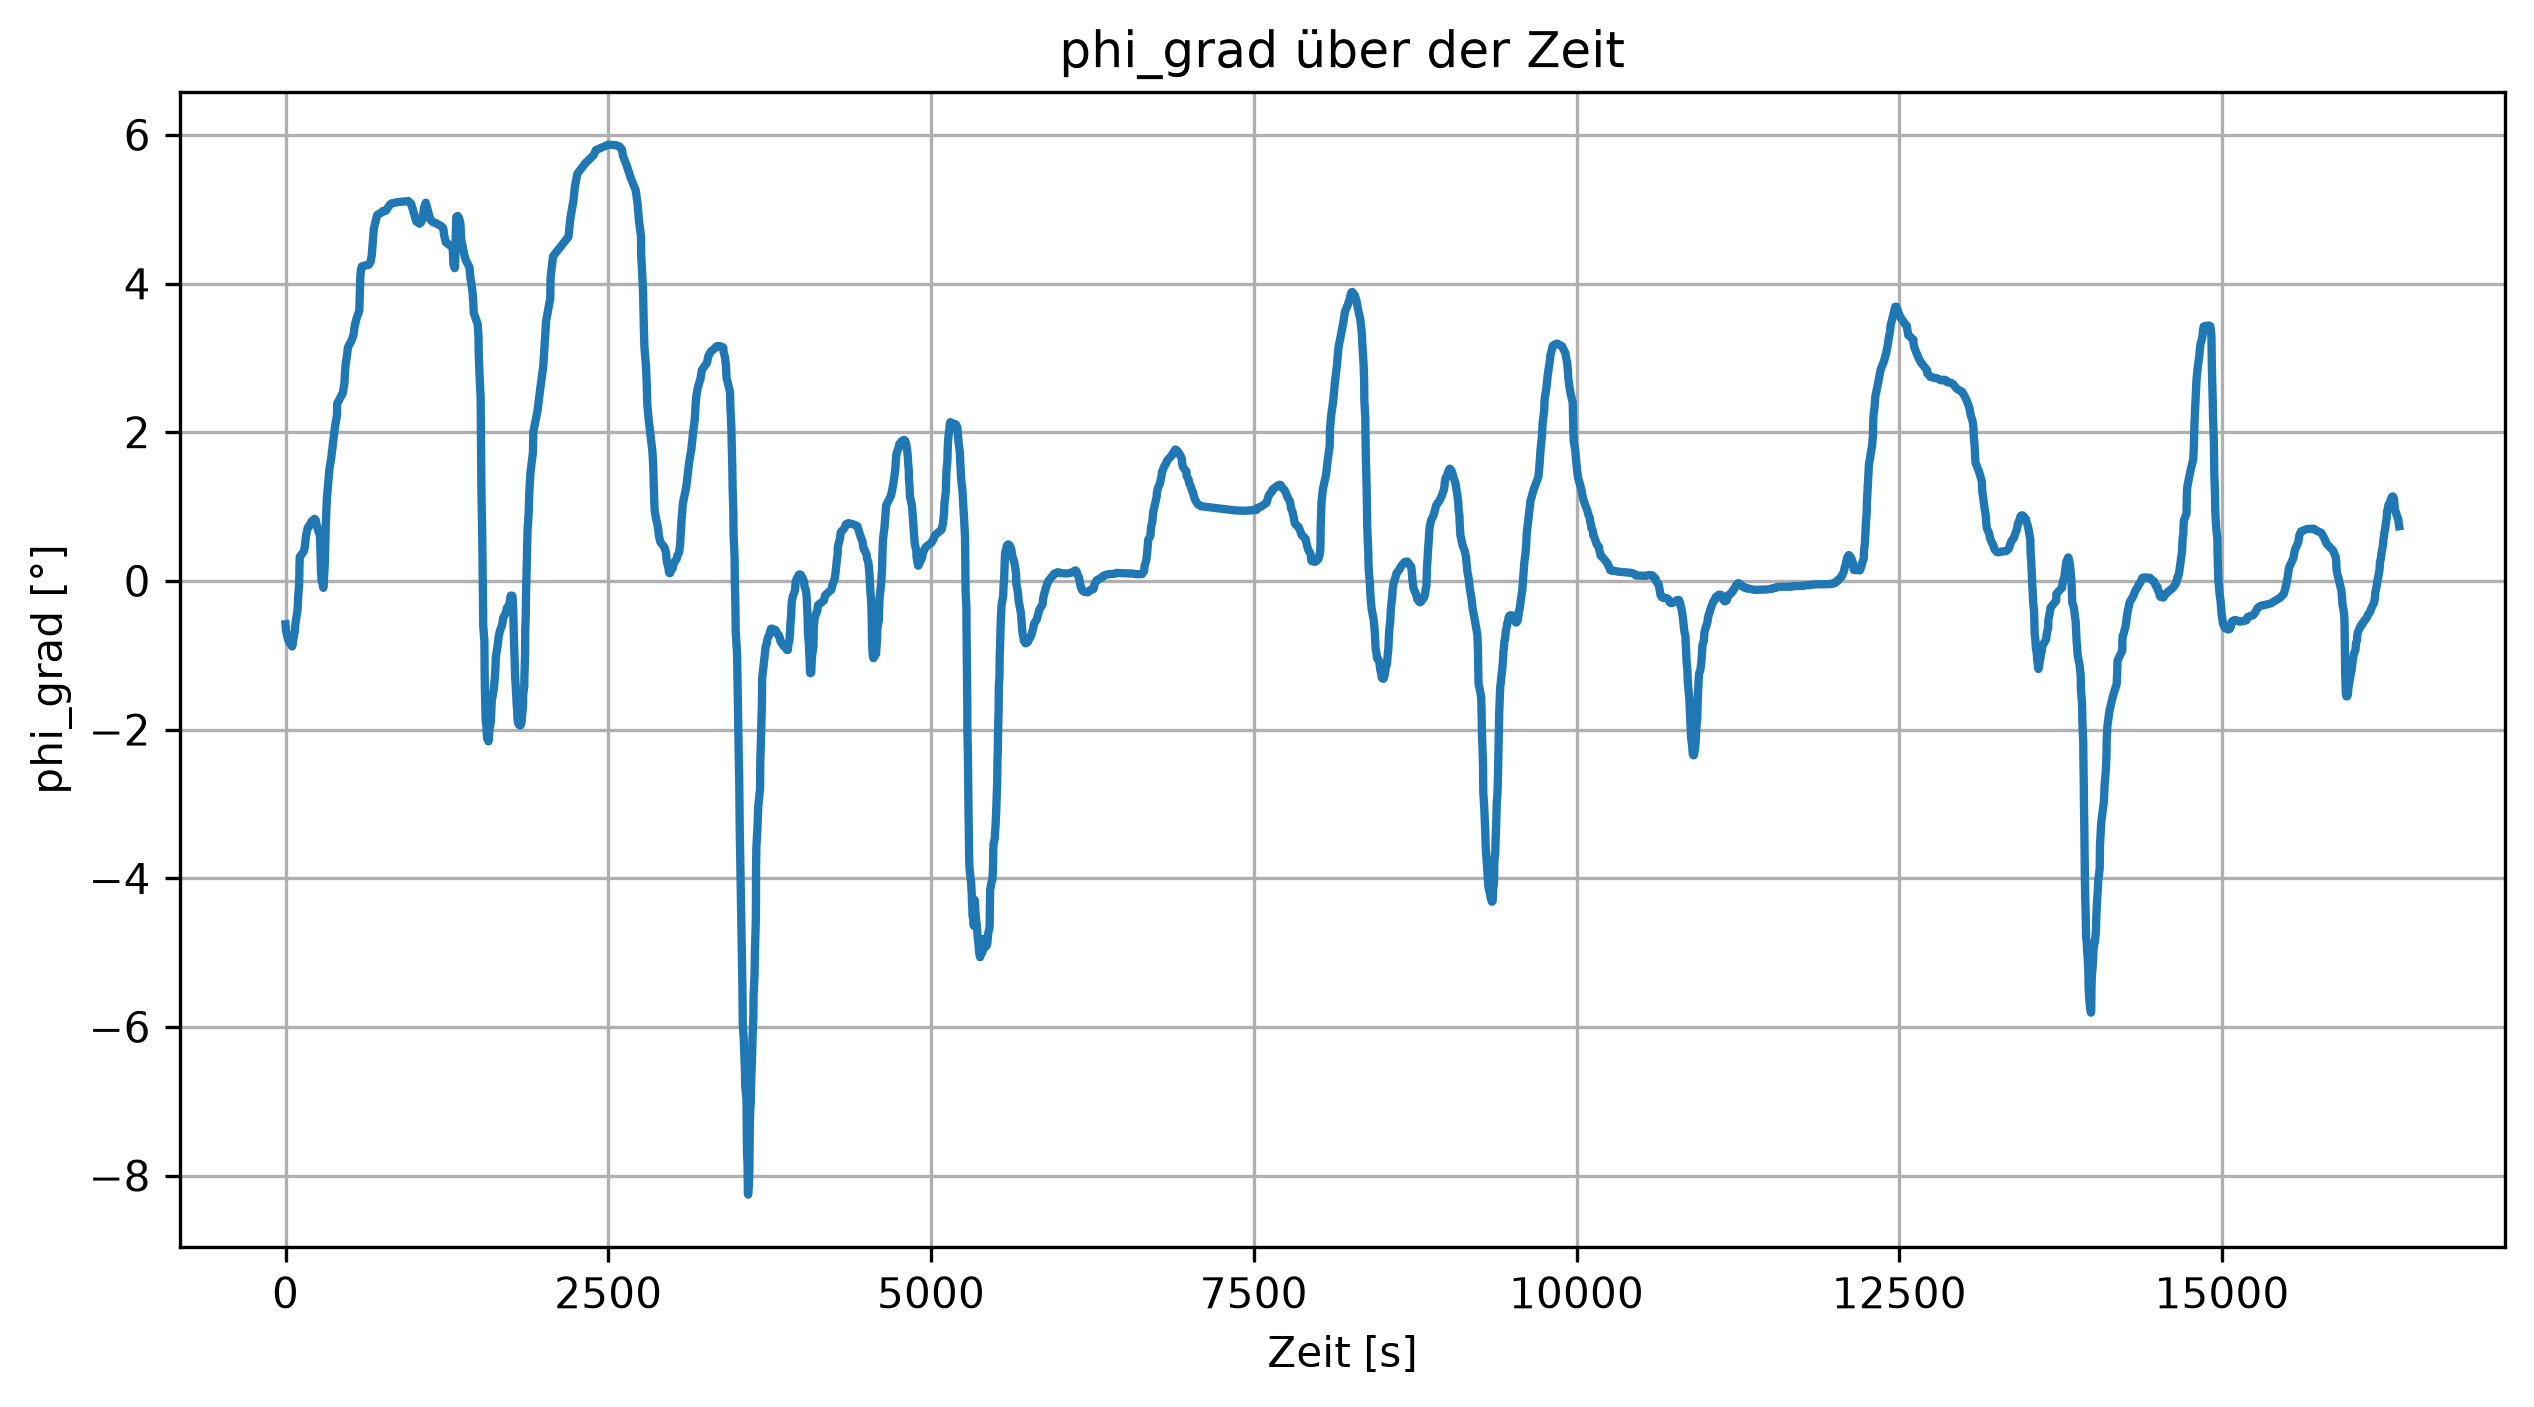
\includegraphics[width=0.95\textwidth]{phi_grad.png}%
\caption{phi\_grad}%
\end{figure}

%
\subsection{plot\_ladezustand}%
\label{subsec:plotladezustand}%


\begin{figure}[H]%
\centering%
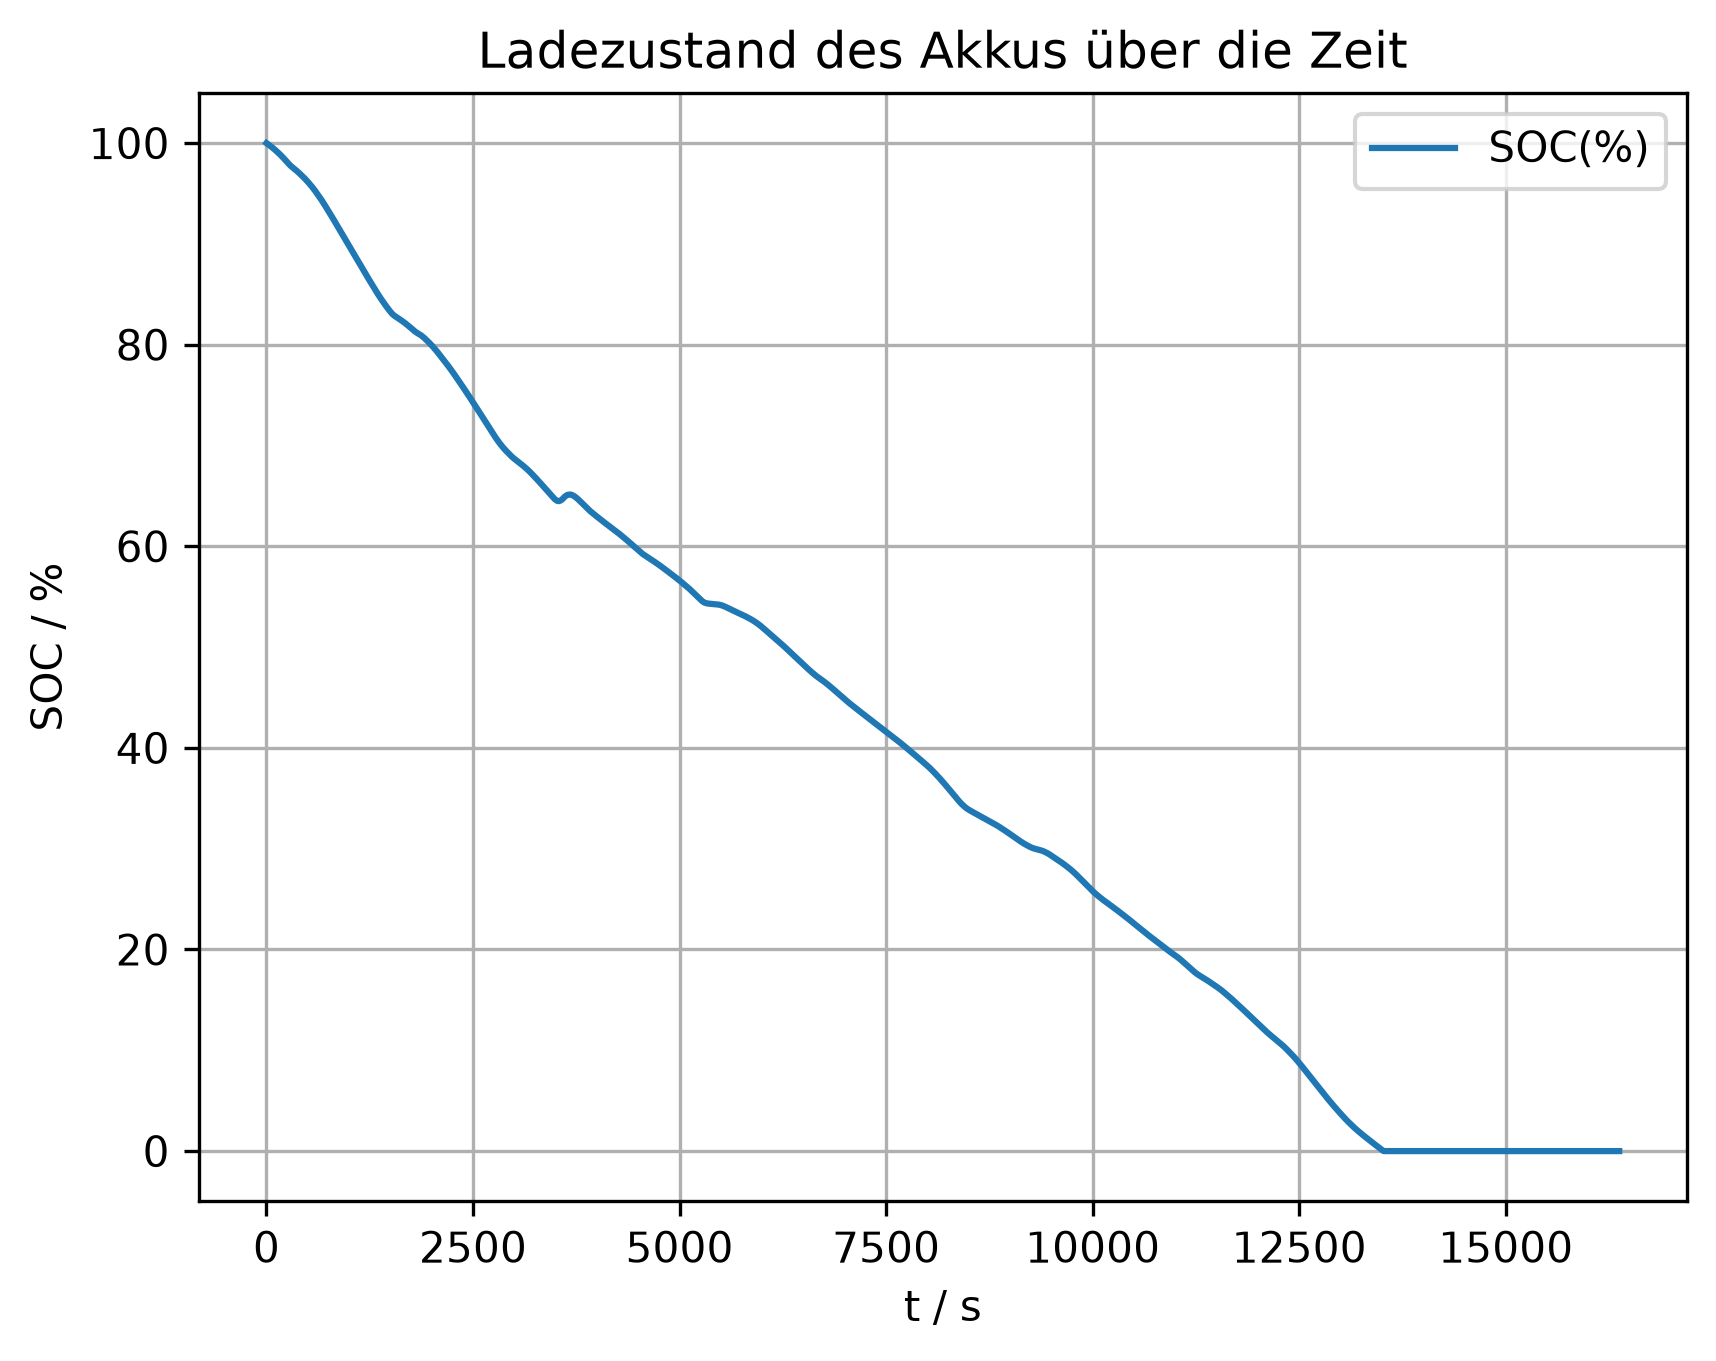
\includegraphics[width=0.95\textwidth]{plot_ladezustand.png}%
\caption{plot\_ladezustand}%
\end{figure}

%
\subsection{rho}%
\label{subsec:rho}%


\begin{figure}[H]%
\centering%
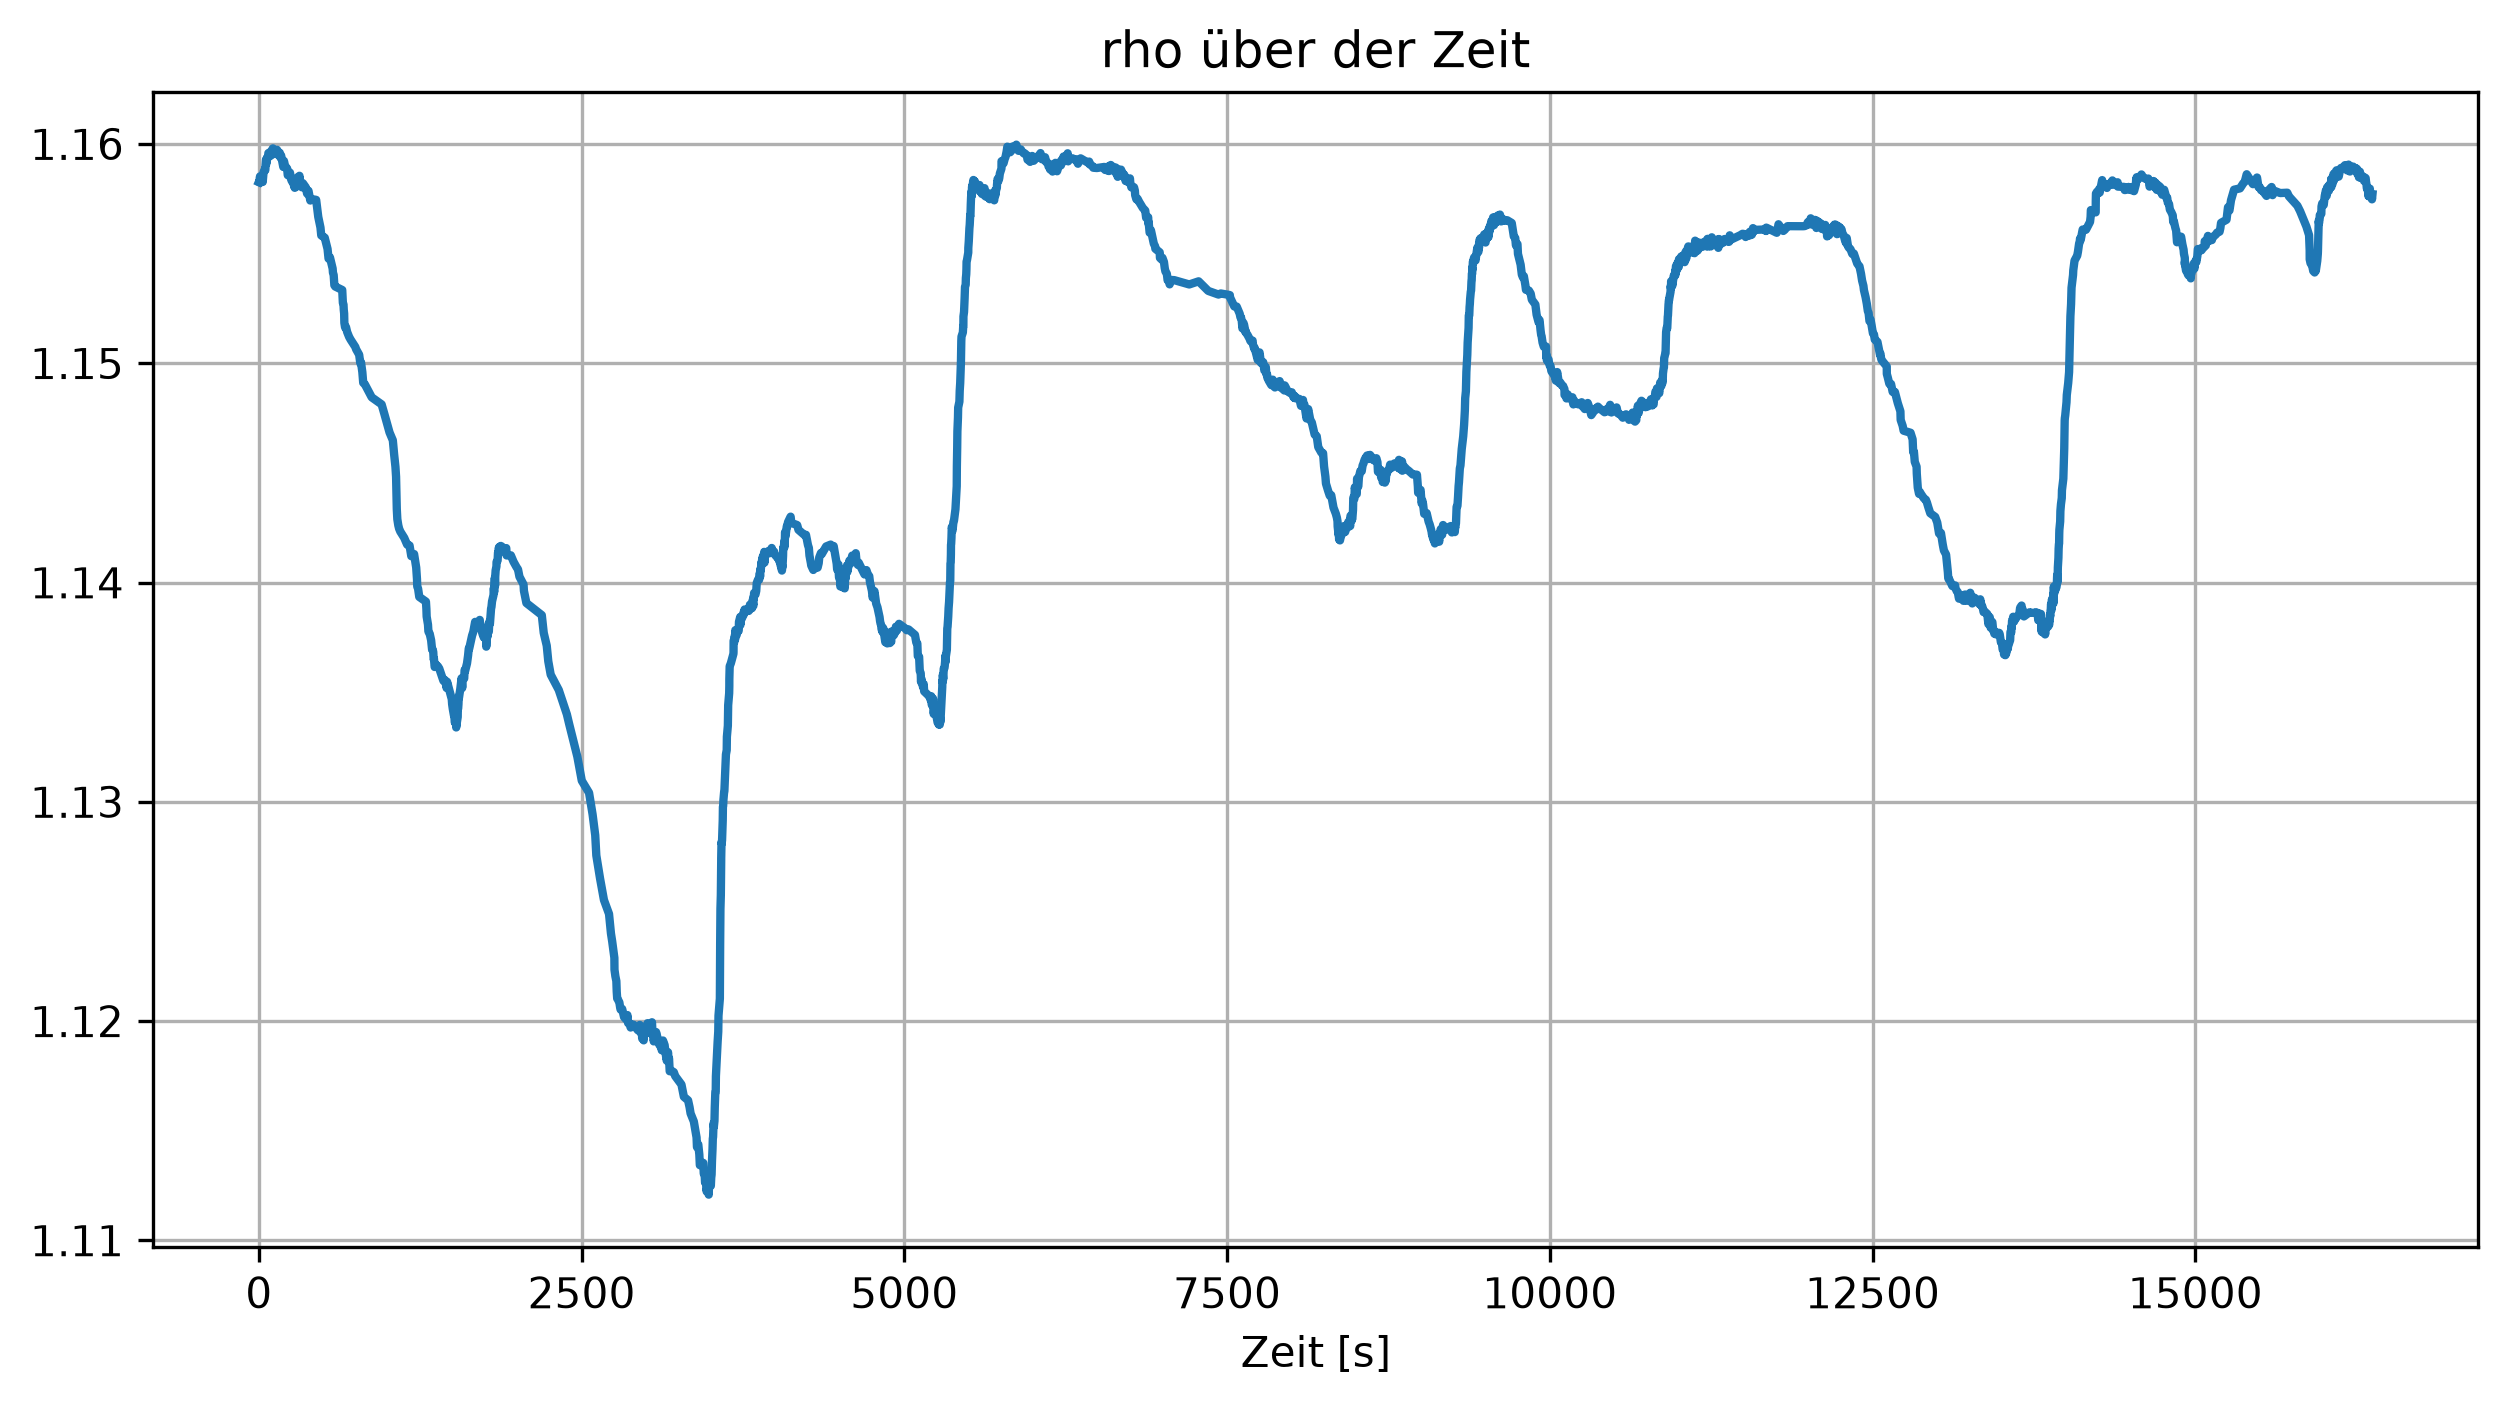
\includegraphics[width=0.95\textwidth]{rho.png}%
\caption{rho}%
\end{figure}

%
\subsection{richtung}%
\label{subsec:richtung}%


\begin{figure}[H]%
\centering%
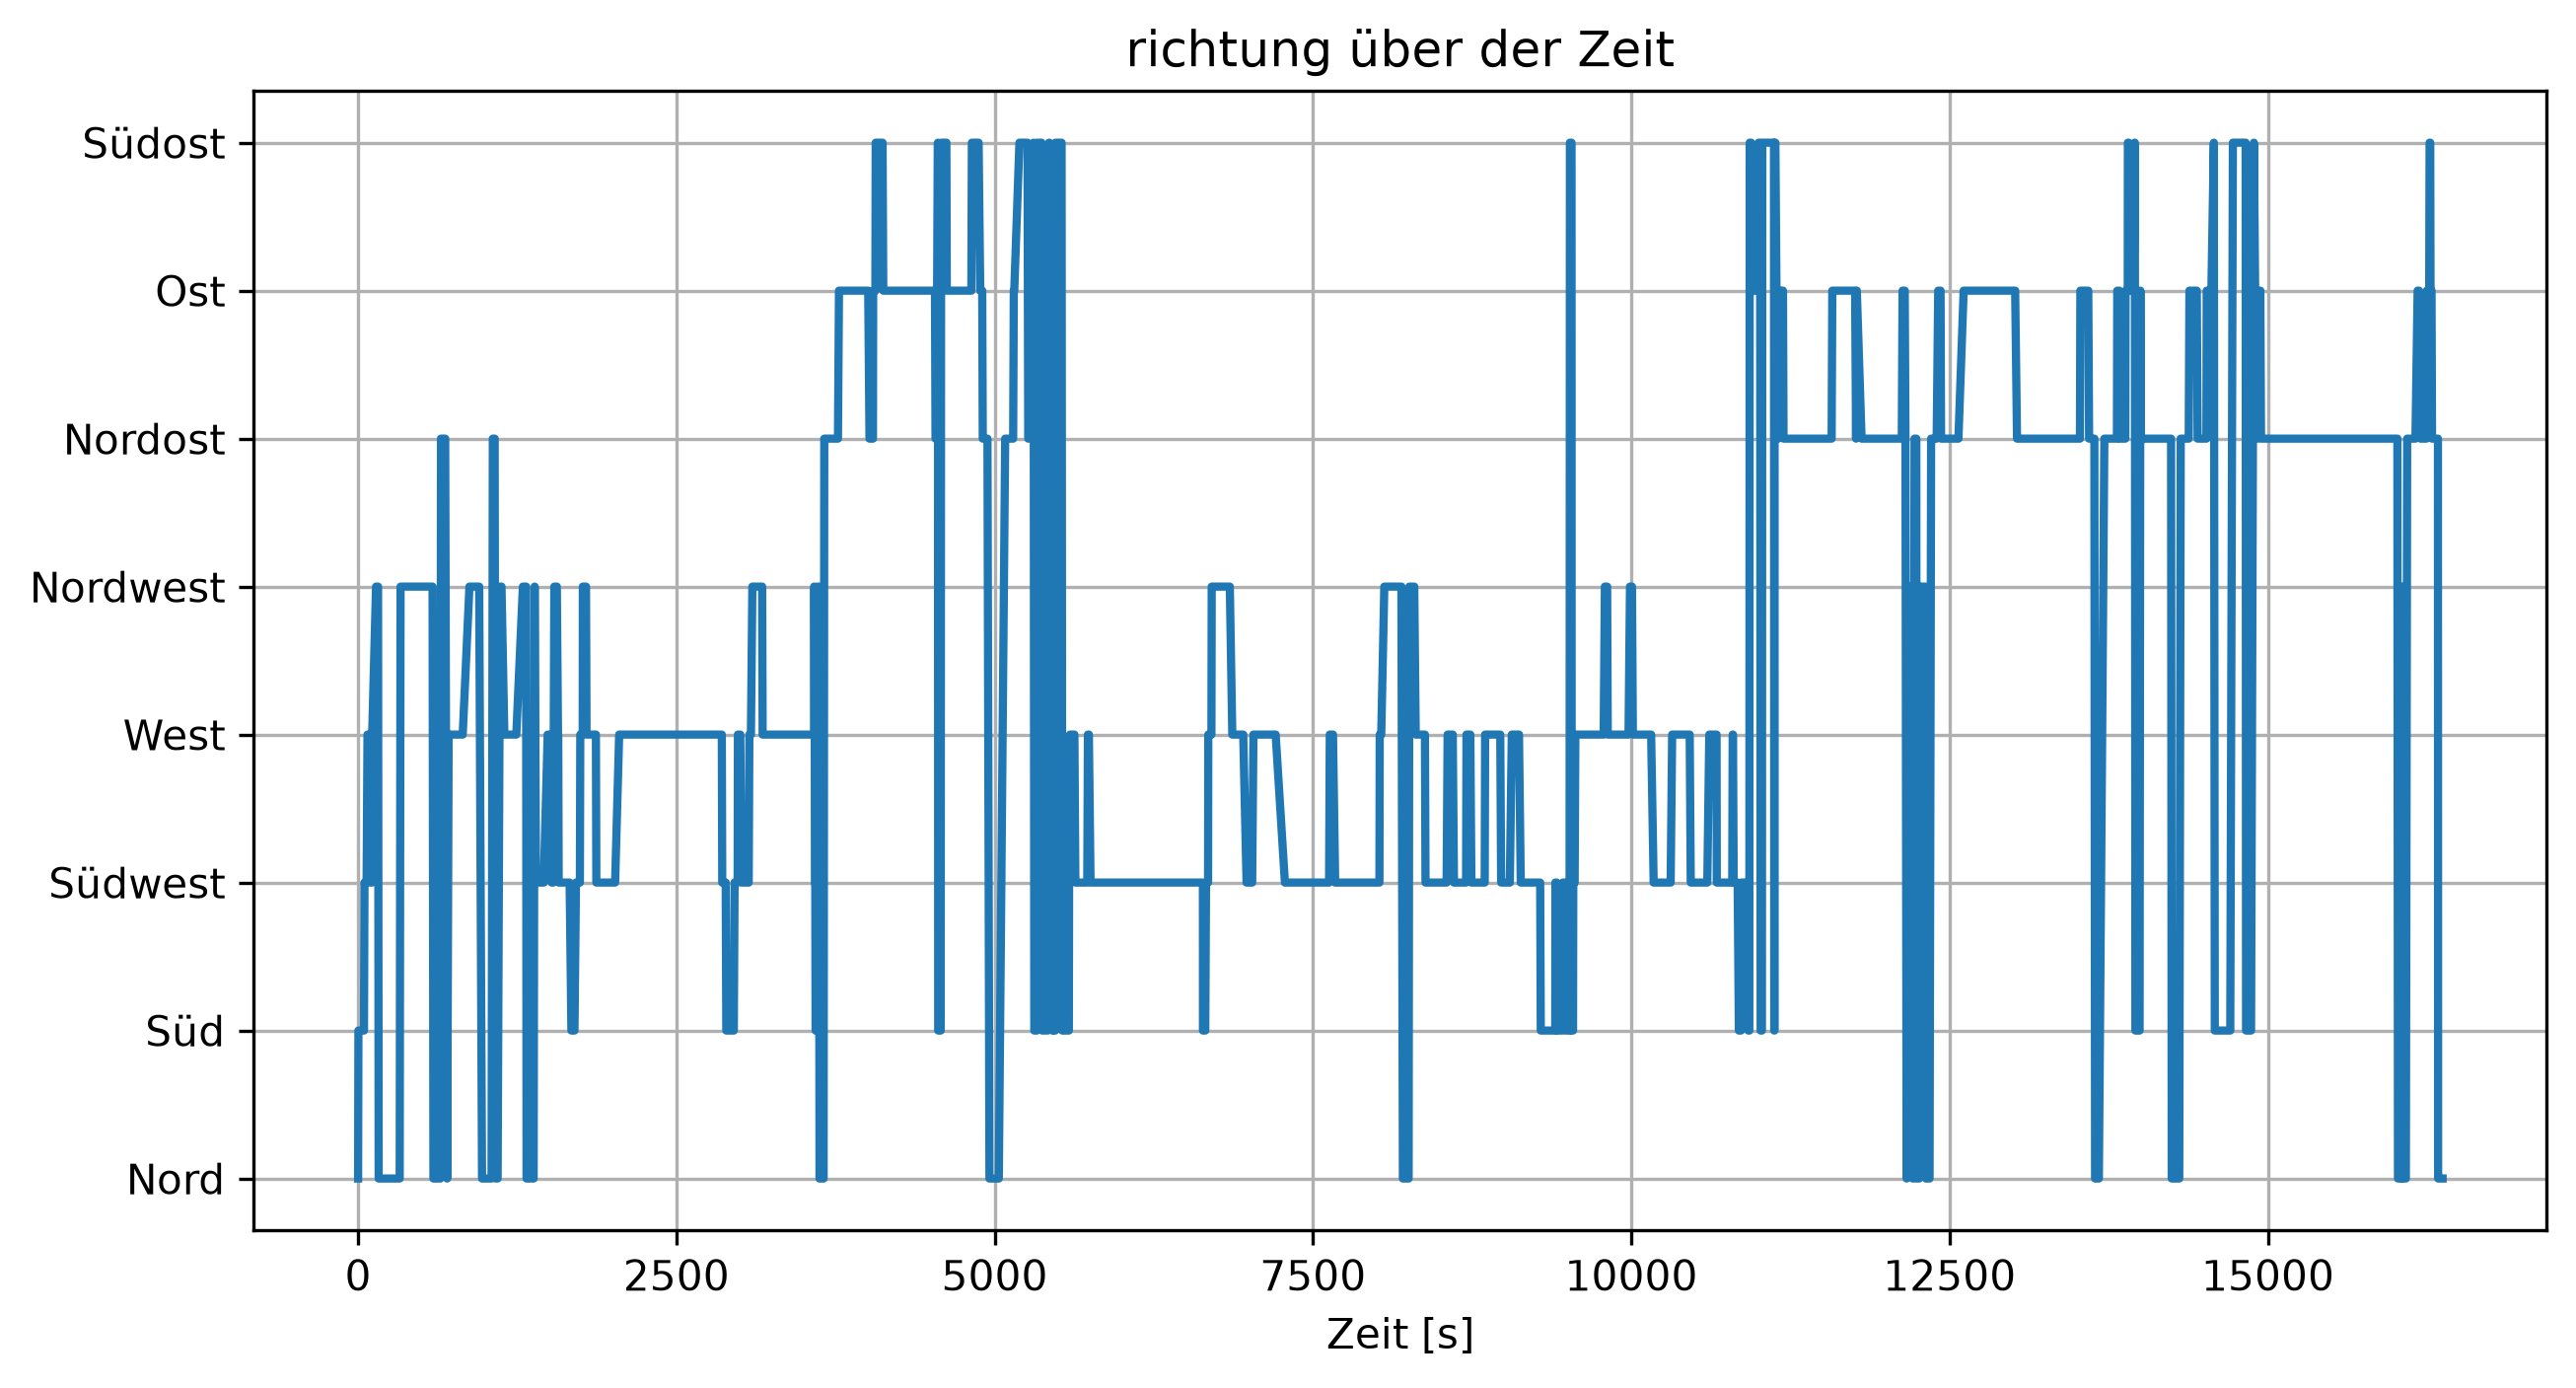
\includegraphics[width=0.95\textwidth]{richtung.png}%
\caption{richtung}%
\end{figure}

%
\subsection{s}%
\label{subsec:s}%


\begin{figure}[H]%
\centering%
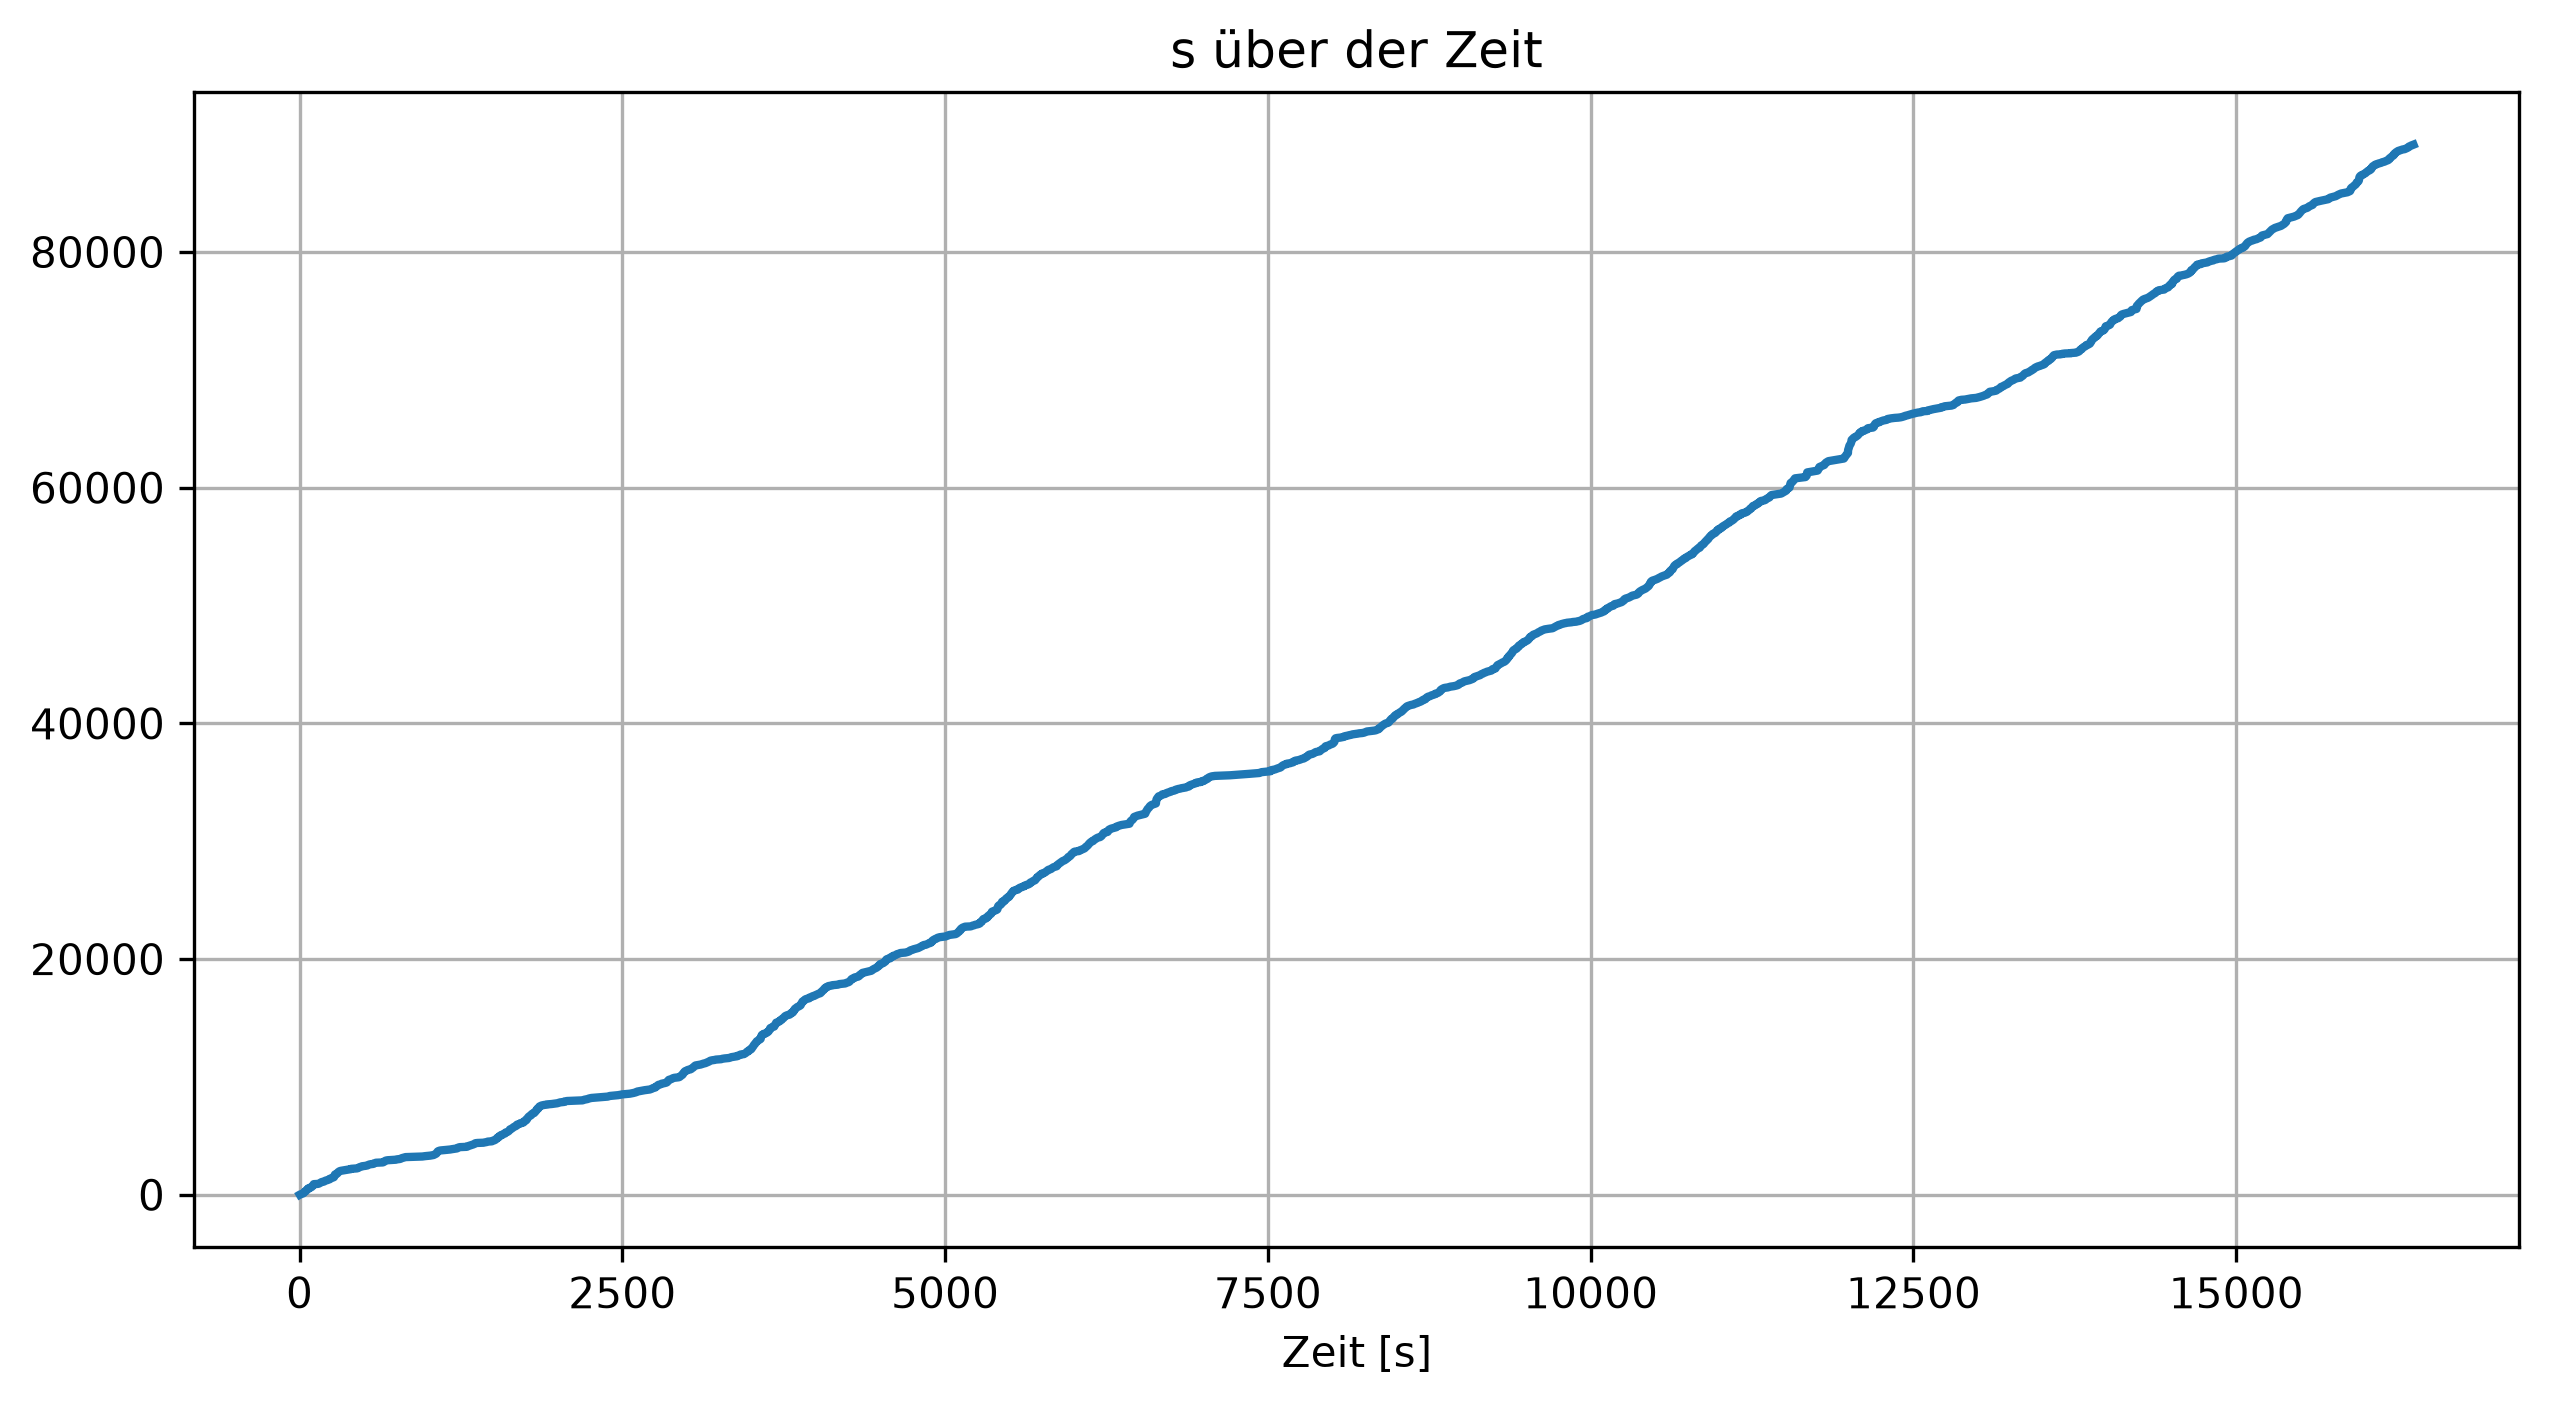
\includegraphics[width=0.95\textwidth]{s.png}%
\caption{s}%
\end{figure}

%
\subsection{s\_orig}%
\label{subsec:sorig}%


\begin{figure}[H]%
\centering%
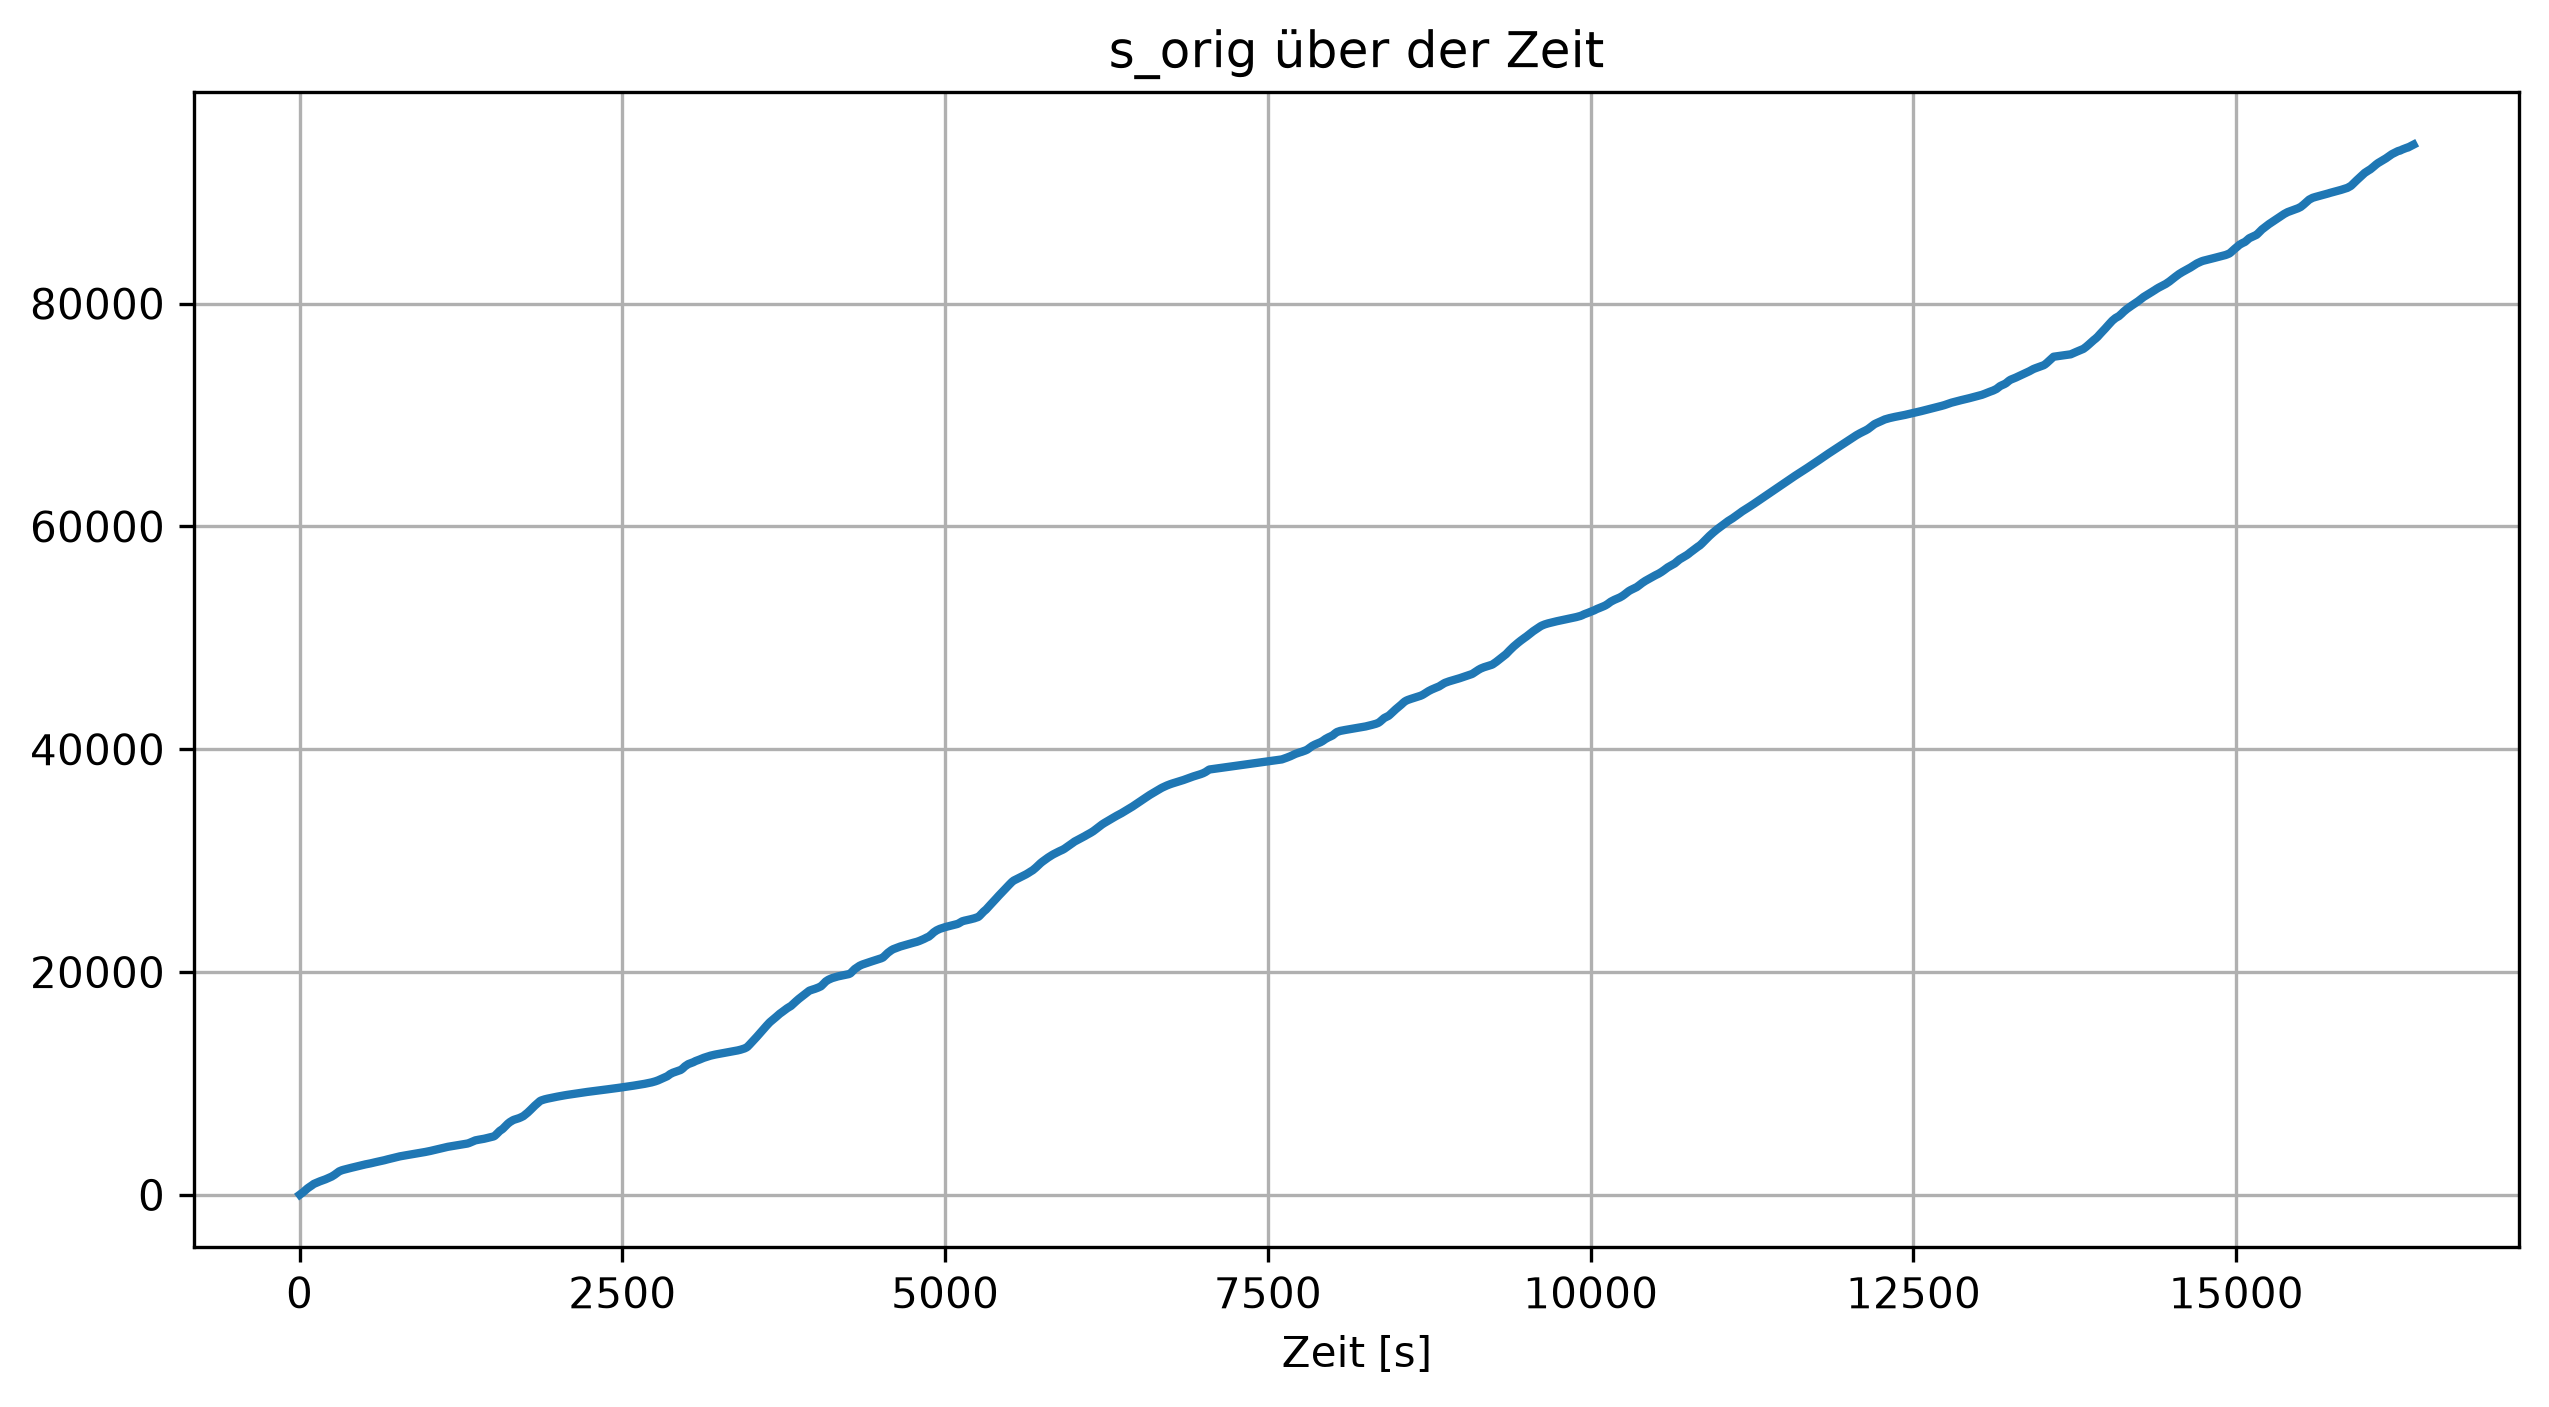
\includegraphics[width=0.95\textwidth]{s_orig.png}%
\caption{s\_orig}%
\end{figure}

%
\subsection{temperature}%
\label{subsec:temperature}%


\begin{figure}[H]%
\centering%
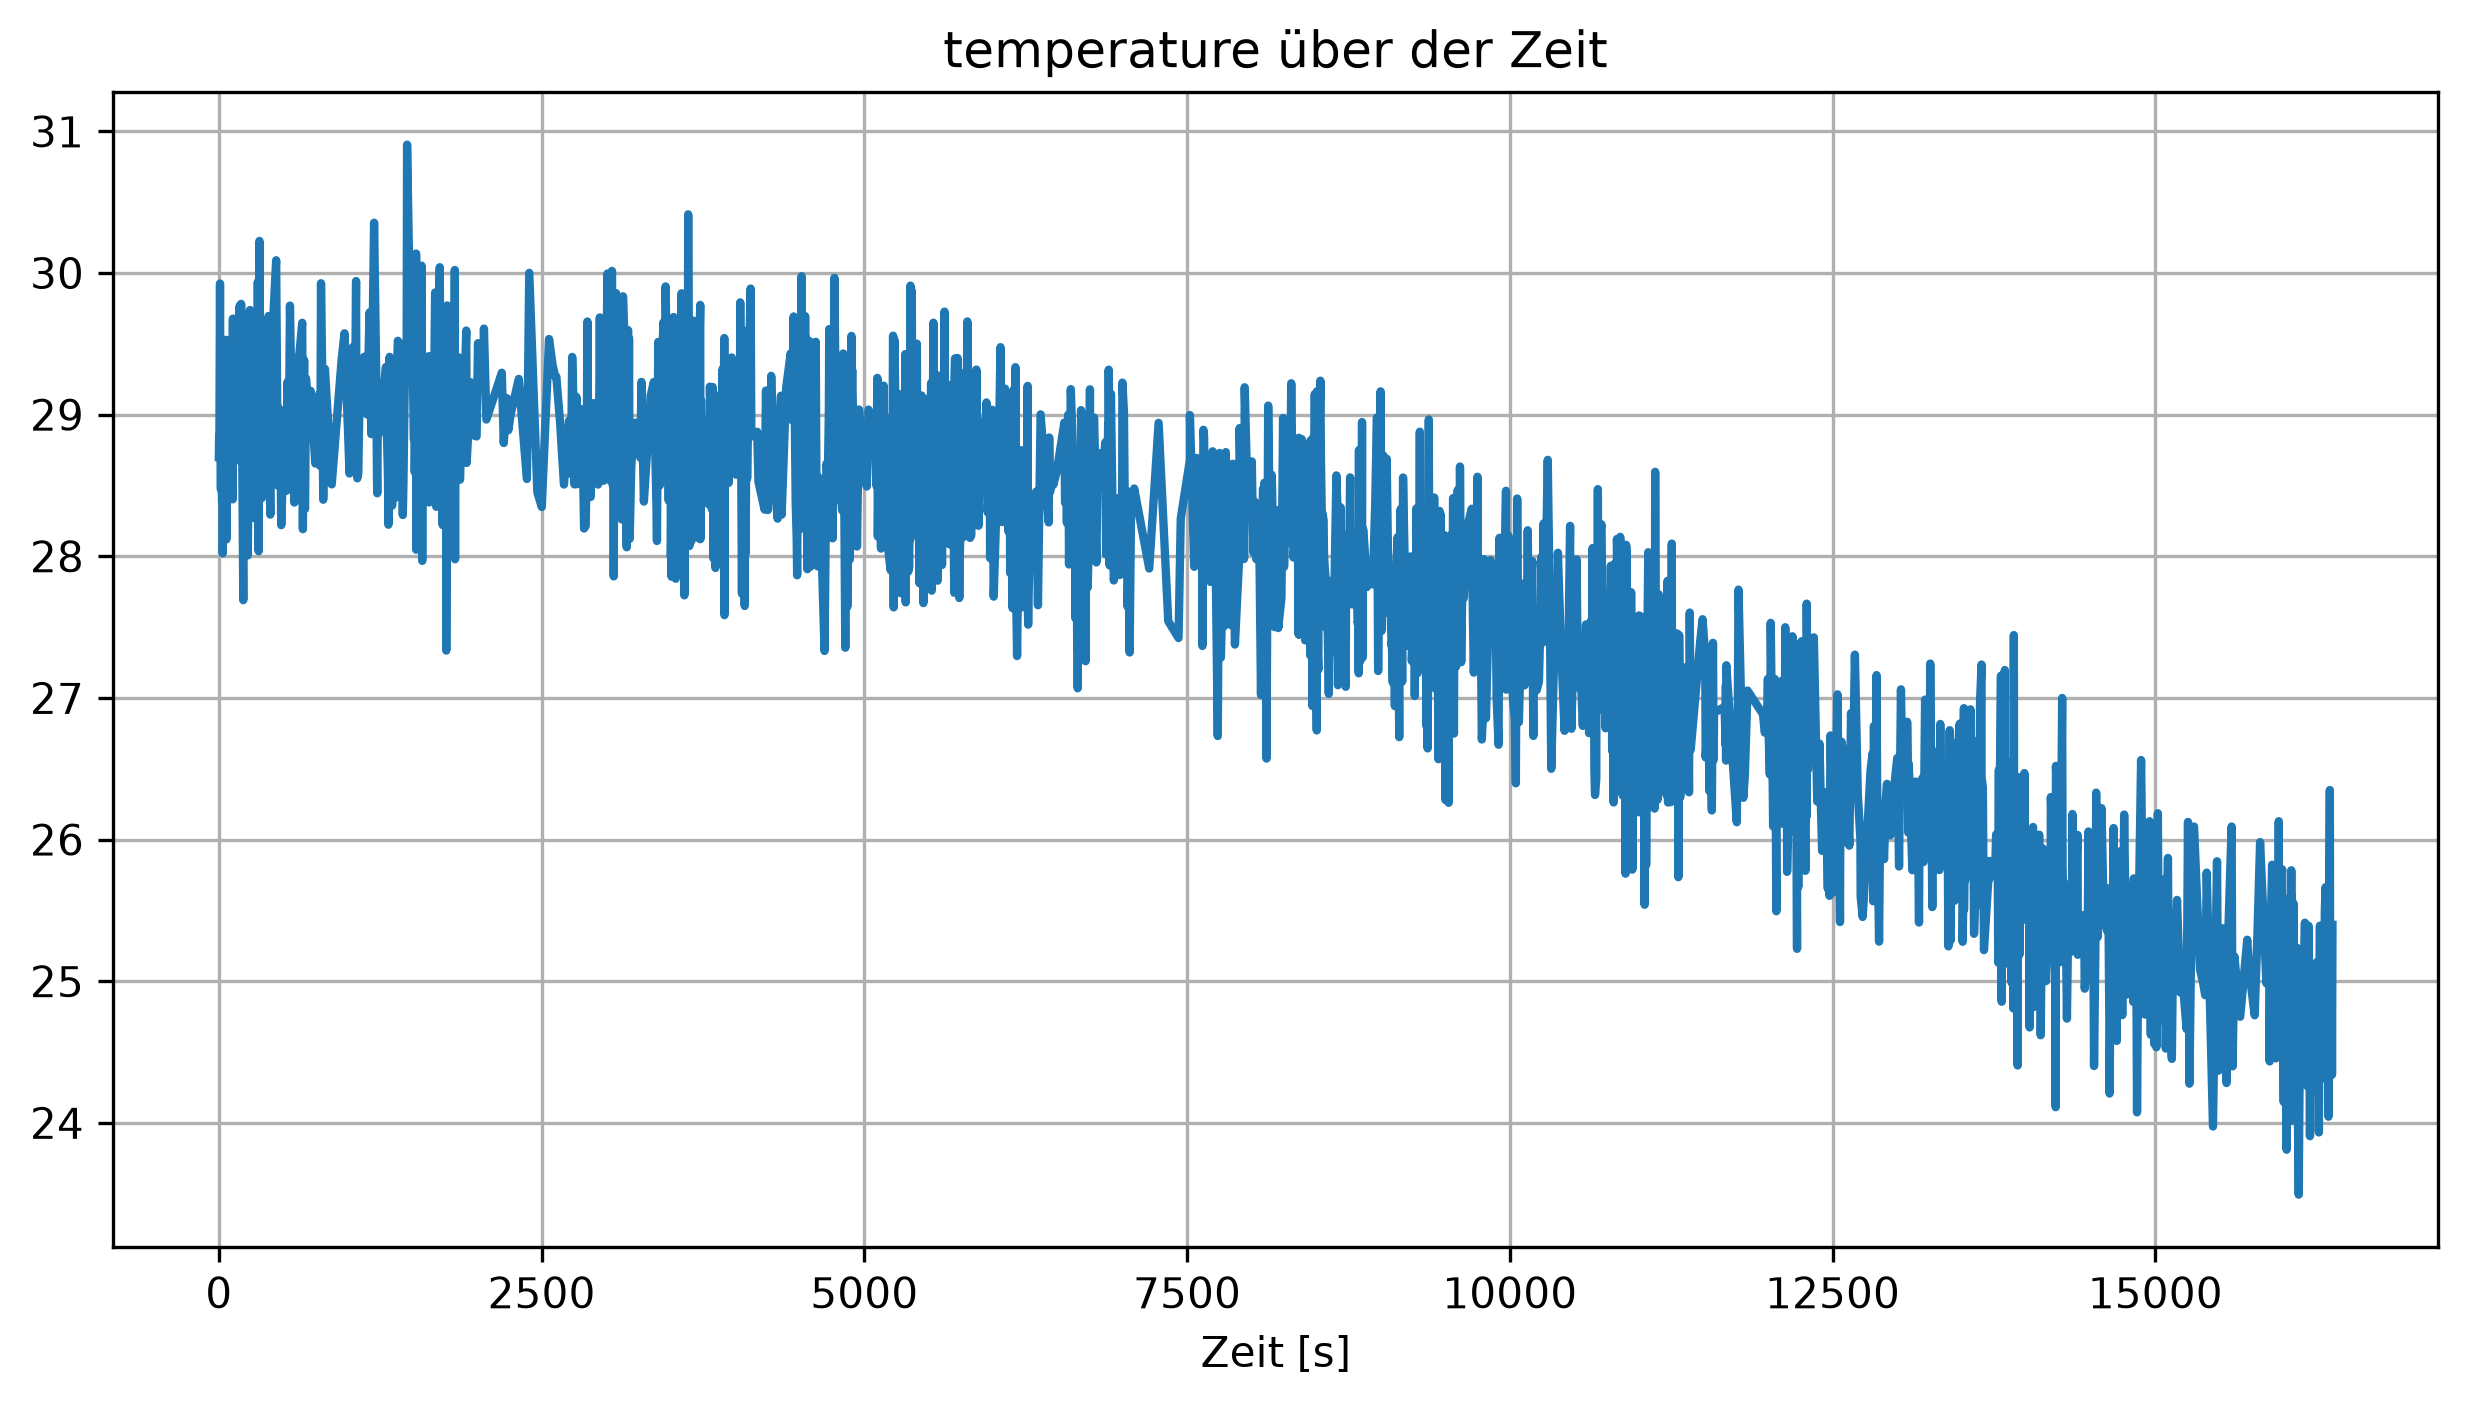
\includegraphics[width=0.95\textwidth]{temperature.png}%
\caption{temperature}%
\end{figure}

%
\subsection{v}%
\label{subsec:v}%


\begin{figure}[H]%
\centering%
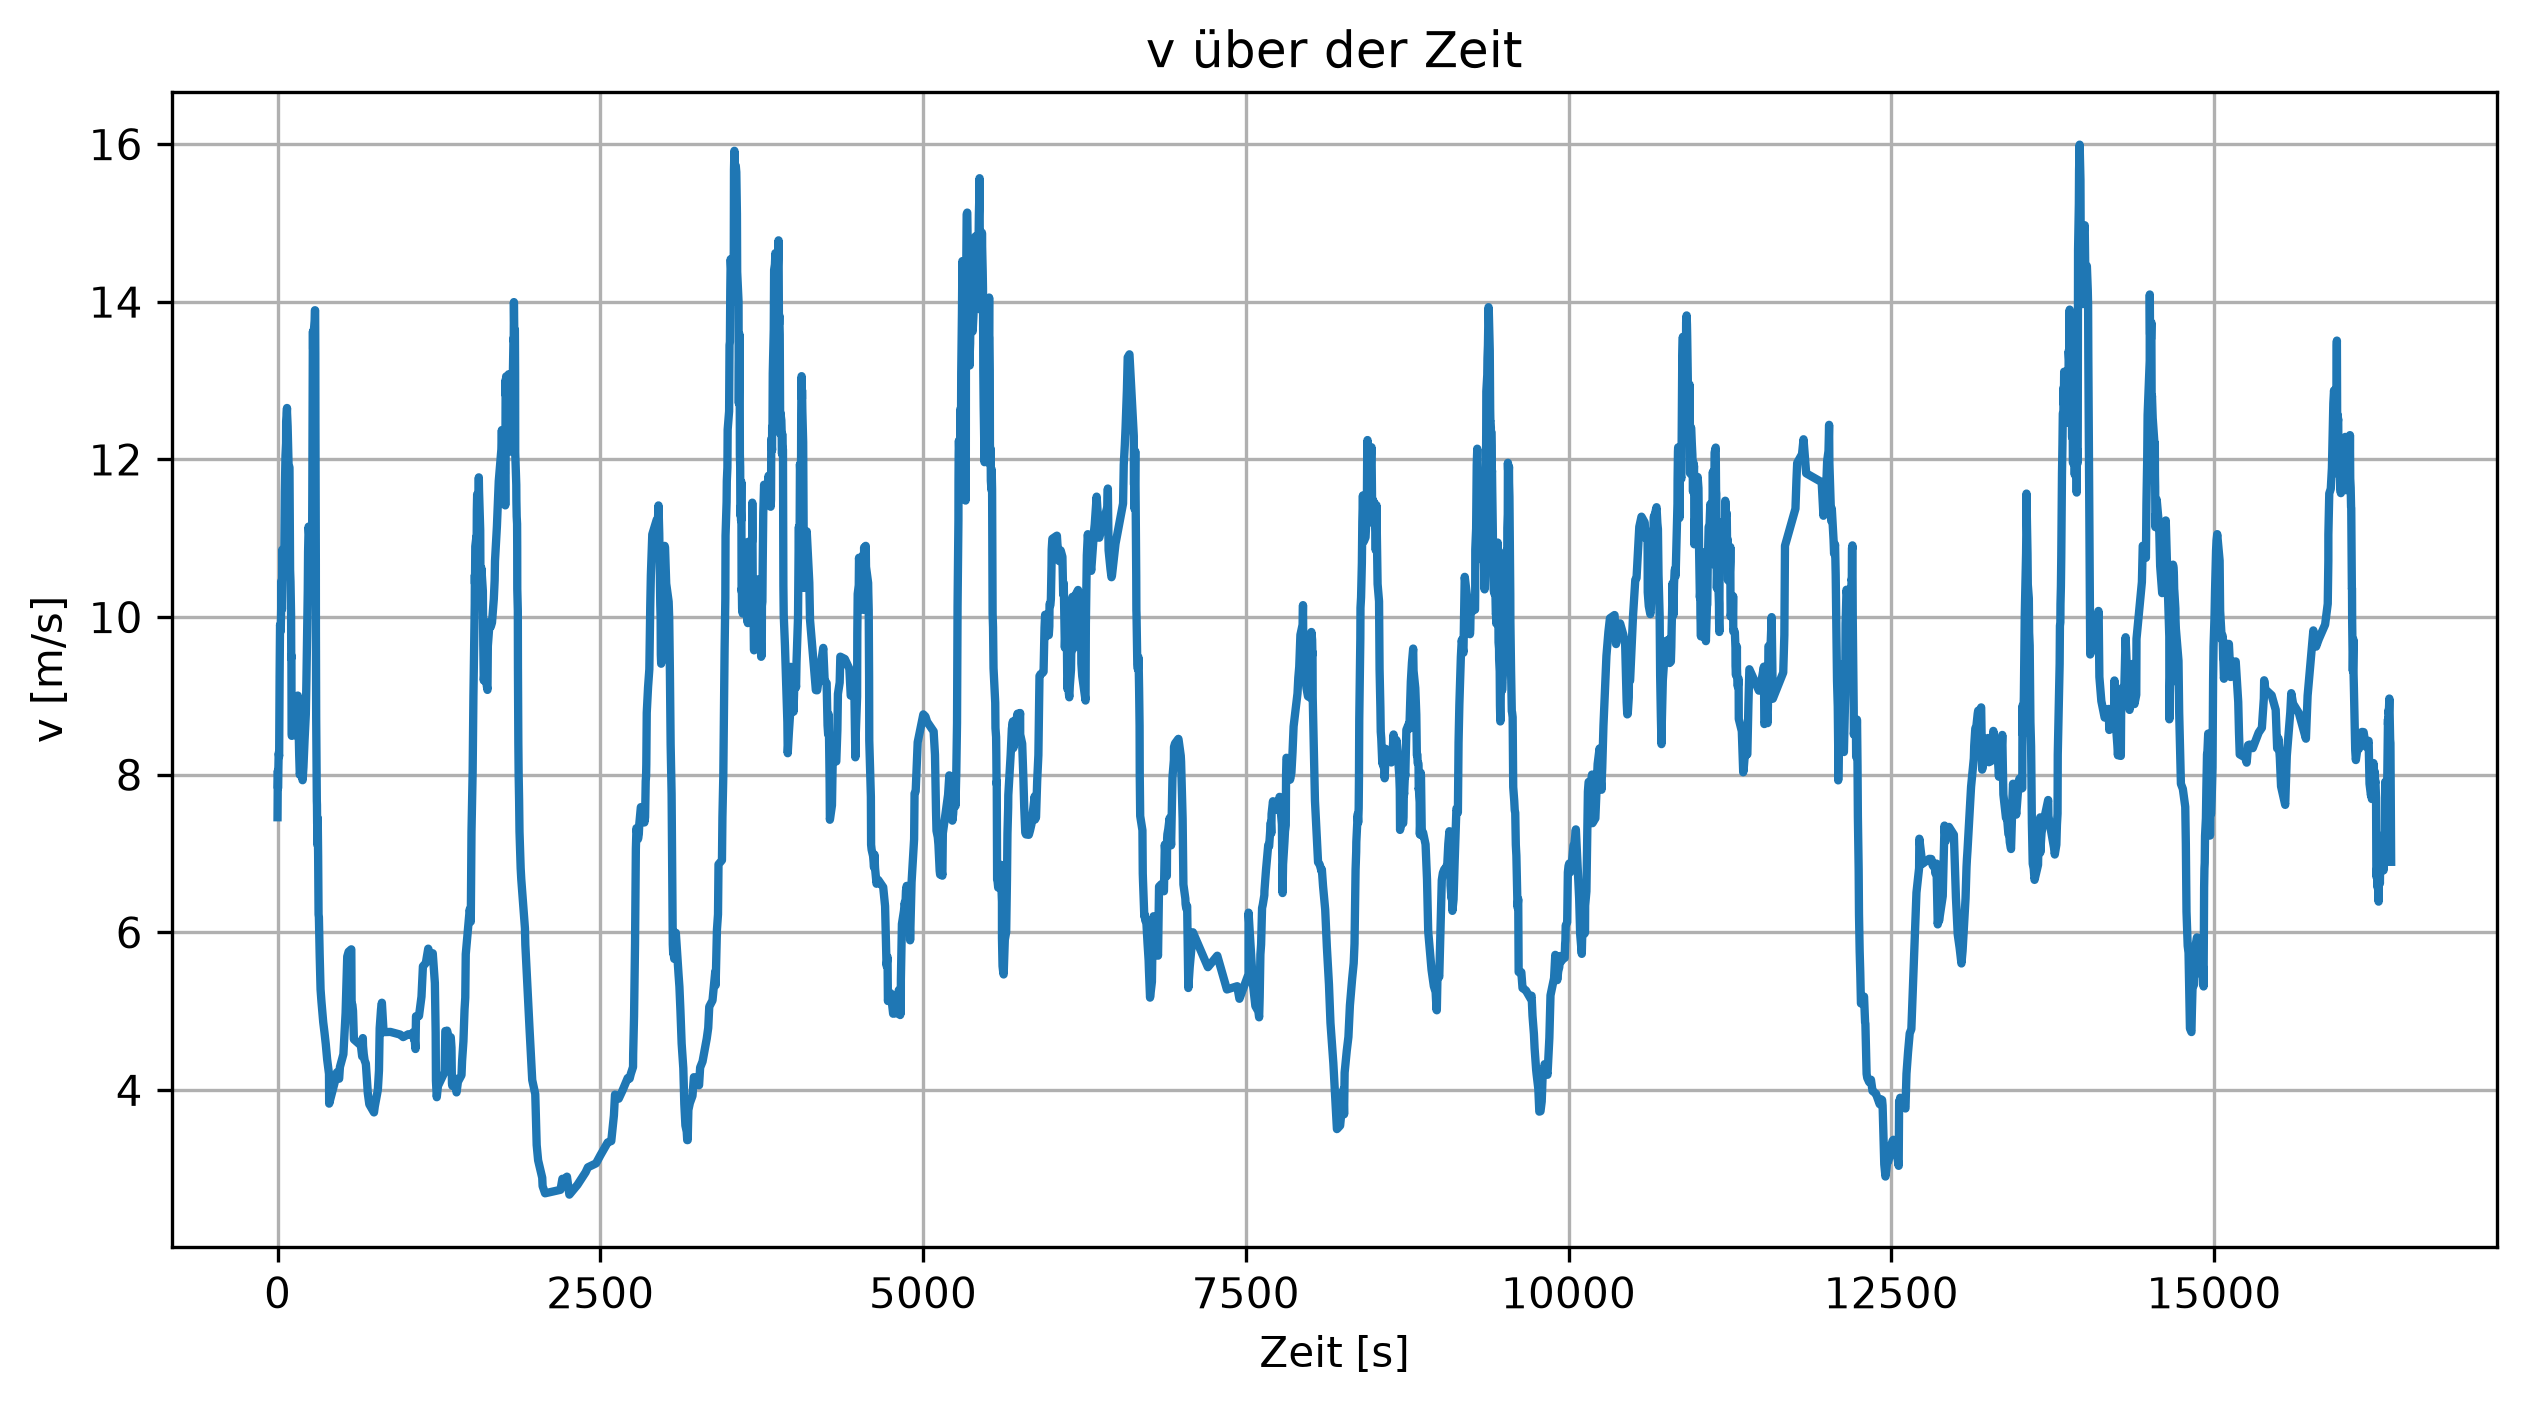
\includegraphics[width=0.95\textwidth]{v.png}%
\caption{v}%
\end{figure}

%
\end{document}